\documentclass{report}

\usepackage{amsmath}
\usepackage{amssymb}
\usepackage{amsthm}
\usepackage{array}
\usepackage{mathtools}
\usepackage{titlepic}
\usepackage{url}
\usepackage{natbib}
\usepackage{graphicx}
\usepackage{epsfig}
\usepackage{listings}
\usepackage{color}
\usepackage{courier}
\usepackage{lmodern}
\usepackage{xfrac}
\usepackage{mdframed}
\usepackage[T1]{fontenc}

\allowdisplaybreaks
\setlength\parindent{0pt}
\graphicspath{{./images/}}

\definecolor{ggreen}{rgb}{0,0.6,0}
\definecolor{mygray}{rgb}{0.5,0.5,0.5}
\definecolor{mmauve}{rgb}{0.58,0,0.82}
\definecolor{backcolour}{rgb}{0.95,0.95,0.92}

\lstset{
	basicstyle=\footnotesize\ttfamily,
	numbers=left,
	stepnumber=1,
	numbersep=5pt,
	numberstyle=\small\ttfamily\color{black},
	breaklines=true,
	showstringspaces=false,
	tabsize=2,
	captionpos=b,
	commentstyle=\color{ggreen},
	escapeinside={\%*}{*)},
	keywordstyle=\color{blue},
	stringstyle=\color{mmauve},
	backgroundcolor=\color{backcolour}, 
}

%\setlength{\tabcolsep}{20pt}
%\renewcommand{\arraystretch}{1.5}

\renewcommand{\baselinestretch}{1.5}

\newtheorem*{theorem}{Theorem}
\newtheorem*{lemma}{Lemma}



\begin{document}

\titlepic{\includegraphics[scale=0.5]{DIT_logo}}
\title{The Parking Problem}
\author{Jerry Kiely\\
	\\
	School of Mathematical Sciences\\
	Dublin Institute of Technology\\
	Dublin 8\\
	Ireland\\
	\\
	\texttt{d16126734@mydit.ie}}
\date{\today}
\maketitle



\tableofcontents


\newpage



%\begin{minipage}[b]{1\linewidth}
    \listoffigures
%\end{minipage}

%\begin{minipage}[b]{1\linewidth}
    \listoftables
%\end{minipage}

%\begin{minipage}[b]{1\linewidth}
	\lstlistoflistings
%\end{minipage}




\newpage




\begin{abstract}
The \emph{parking problem} was proposed by Alfred R\'{e}nyi in 1958 - cars, modelled 
as unit intervals, are placed at random upon a street of length $x$ until no spaces 
that can accommodate cars remain. R\'{e}nyi showed that the \emph{jamming limit}, or 
expected coverage of cars on the street, is approximately $75\%$.\bigskip

As well as being an interesting problem in it's own right, applications of the parking 
problem are numerous in physics and chemistry. One of the most interesting applications 
is in the theory of \emph{Random Sequential Adsorption}, or RSA, which models the 
surface deposition of particles upon a substrate.\bigskip

There are a number of approaches to this problem in one dimensions. In this paper we 
will look at three of the approaches - an elementary treatment, an approach that makes 
use of Laplace Transforms, and the kinetic approach that looks at the time evolution 
of the line filling process.\bigskip

We will also look at a number of different generalizations of the problem, including 
\emph{parking with overlap}, also know as \emph{cooperative} RSA, and 
\emph{the reversible parking problem}, where cars arrive and leave at different rates.
\end{abstract}



%\renewcommand{\abstractname}{Acknowledgements}
%\begin{abstract}
%	I would like to thank Dana Mackey for her help, advice, and feedback.
%\end{abstract}





\chapter{Introduction}











\section{Problem Statement}

Consider an interval $(0, x)$ upon which we place a segment of unit length 
at random. We continue by placing a second segment of unit length randomly 
upon the original interval, discarding the segment if it overlaps with the 
original one. \bigskip

We continue in this fashion until we can no longer add unit segments without 
overlap. At each step the next position within the interval is chosen from a 
uniform distribution of the remaining locations within the interval. \bigskip

We are interested in both the expected value of the number of unit segments 
contained within the interval $(0, x)$, denoted $M(x)$, and the expected 
filling density of unit segments within the interval, denoted $M(x) / x$. \bigskip






\section{Derivation of the Master Equation}

We first look at the derivation of the master equation for $M(x)$ which forms the 
heart of the problem, and will be crop up in the rest of the paper. \bigskip

We initially consider an interval $(0, x + 1)$ and upon this place a unit segment 
$(t, t + 1)$. This unit segment partitions the original interval into two smaller 
intervals - $(0, t)$ and $(t + 1, x + 1)$. The expected number of unit segments 
contained within the original interval is: \bigskip

\[
	M(x + 1) = M(t) + 1 + M(x - t)
\]\medskip

where $1$ represents the expectation of the added segment within the unit interval 
$(t, t + 1)$ - in other words, we have one unit segment within the unit interval 
$(t, t + 1)$. Integrating with respect to $t$ we get: \bigskip

\begin{eqnarray*}
	\int_{0}^{x} M(x + 1) dt & = & \int_{0}^{x} [M(t) + 1 + M(x - t)] dt \\\\
	M(x + 1) \int_{0}^{x} dt & = & \int_{0}^{x} dt + \int_{0}^{x} [M(t) + M(x - t)] dt \\\\
			M(x + 1) \cdot x & = & x + \int_{0}^{x} [M(t) + M(x - t)] dt \\\\
					M(x + 1) & = & 1 + \frac{1}{x} \int_{0}^{x} [M(t) + M(x - t)] dt 
\end{eqnarray*}\medskip

as the distributions within each of the smaller intervals are uniform, and hence 
the same, we get: \bigskip

\begin{eqnarray} \label{eq:1}
	M(x + 1) = 1 + \frac{2}{x} \int_{0}^{x} M(t) dt
\end{eqnarray}\medskip

changing variables we get: \bigskip

\begin{eqnarray} \label{eq:2}
	M(x) = 1 + \frac{2}{x - 1} \int_{0}^{x - 1} M(t) dt
\end{eqnarray}\medskip

more completely, and because adding a unit segment to an interval of length less 
than $1$ has no meaning, the equation for $M(x)$ can be written as follows: \bigskip

\begin{eqnarray} \label{eq:3}
	M(x) = 
	\begin{dcases}
		0,                                            & \text{for } 0 \leq x < 1 \\\\
		1,                                            & \text{for } x = 1 \\\\
		1 + \frac{2}{x - 1} \int_{0}^{x - 1} M(t) dt, & \text{for } x > 1
	\end{dcases}
\end{eqnarray}\medskip

which has the form of a recurrence. 






\section{Applications}

The main application of the parking problem is to the theory of random 
sequential adsorption (RSA), which models the adsorption of particles onto 
a solid substrate. It is important to make the distinction between 
\emph{adsorption} and \emph{absorption} - adsorption involves the surface 
of the material involved, whereas absorption involves the full volume of 
the material. \bigskip

Some examples of RSA are adsorption of gas molecules, polymer chains, 
latex particles, bacteria, proteins, and colloidal particles (insoluble 
particles contained within a suspension) onto a surface. Another important 
application is when applied to genome sequencing where a newly-arriving 
sequenced clone is allowed to partially overlap an existing sequenced 
clone - in which case the parking problem with overlap the most relevant 
model. In some cases adsorbed particles can also be released from a 
surface, a process know as \emph{desorption}, and in this case the 
reversible parking problem is the most relevant model. \bigskip

In order to maximize the adsorption of particles, a clear understanding of 
the problem is required, and to that end we need to be able to faithfully 
model the process. This paper will offer a survey of the approaches to 
modelling the one-dimensional parking problem, and provide a different 
approach to both validate the approaches used to model the process, and to 
calculate the associated constants. \bigskip














\chapter{Weiner's Approach}











\section{Finding the Jamming Limit}

We first look at Weiner's elementary approach to finding the jamming limit $C_R$ 
(see \cite{weiner1969elementary}). Using our previously derived master equation 
(\ref{eq:3}) Weiner solved for $M(x)$ recursively, giving us the following 
results: \bigskip

\begin{eqnarray} \label{eq:4}
	M(x) = 
	\begin{dcases}
		0                                   & \text{if } x \in [0, 1) \\\\
		1                                   & \text{if } x \in [1, 2) \\\\
		3 - \frac{2}{x - 1}                 & \text{if } x \in [2, 3) \\\\
		7 - \frac{10 - 4 \ln(x - 2)}{x - 1} & \text{if } x \in [3, 4)
	\end{dcases}
\end{eqnarray}\medskip

\begin{table}[t!]
	\centering
	\begin{tabular}{|c | c|} 
		\hline
		$x$ & $M(x) / x$ \\ [1ex] 
		\hline
		0.99 & 0 \\ 
		1.99 & 0.5025125628 \\ 
		2.99 & 0.6672156769 \\ 
		3.99 & 0.6854478541 \\ 
		4.99 & 0.6969110964 \\ 
		5.99 & 0.7054612992 \\ 
		6.99 & 0.7114892709 \\  
		\hline
	\end{tabular}
	\caption{$M(x) / x$}
	\label{table:1}
\end{table}\medskip

and so on - the calculations becoming increasingly difficult, and frankly tedious, after this point. In 
table \ref{table:1} we have calculated $M(x) / x$ for values of $x$ close to the upper limit of each interval. 
As can be seen, the values of $M(x) / x$ seem to be approaching a limit. This can be seen more clearly in 
figure \ref{fig:rpc1}. \bigskip

\begin{figure}[h!]
	\centering
	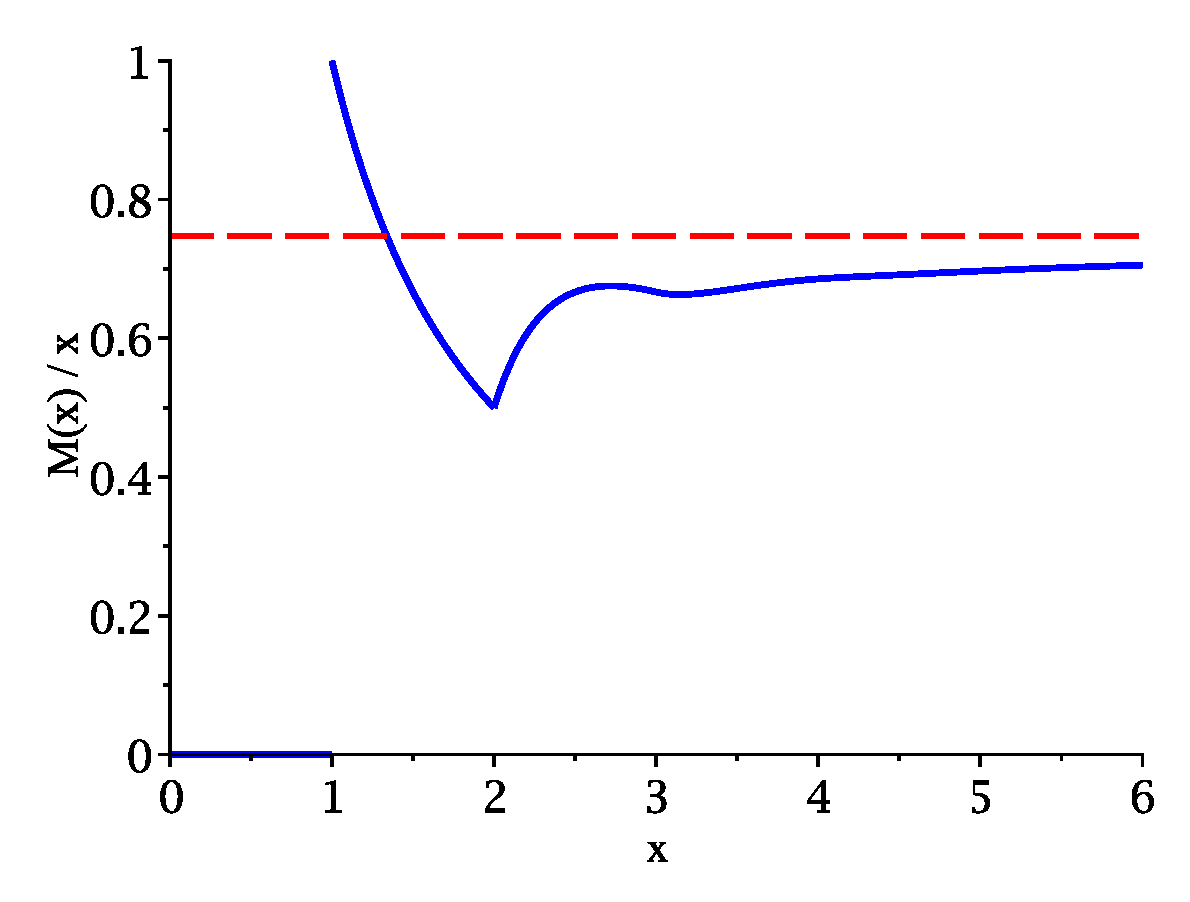
\includegraphics[scale = 0.35]{renyi_01.eps}
	\caption{R\'enyi's parking constant}
	\label{fig:rpc1}
\end{figure}\medskip











\section{Existence of the Jamming Limit}

In attempting to show that this jamming limit exists, Weiner took a flawed approach. In order to understand 
the flaw we trace his steps and return to equation \ref{eq:1}. Dividing across by $x$ we get: \bigskip

\begin{eqnarray} \label{eq:5}
	\frac{M(x + 1)}{x} = \frac{1}{x} + \frac{2}{x^2} \int_{0}^{x} M(t) dt
\end{eqnarray}\medskip

differentiating with respect to $x$: \bigskip

\begin{eqnarray*}
	\left(\frac{M(x + 1)}{x}\right)^{\prime} = -\frac{1}{x^2} - \frac{4}{x^3} \int_{0}^{x} M(t) dt + \frac{2}{x^2} M(x)
\end{eqnarray*}\medskip

looking at the integral, and making use of the fact that $0 \leq M(x) \leq x$ we find that: \bigskip

\begin{eqnarray*} 
	\int_{0}^{x} M(t) dt & \leq & \int_{0}^{x} t dt \\\\
						 & \leq & \frac{x^2}{2}
\end{eqnarray*}\medskip

making use of both we find: \bigskip

\begin{eqnarray*} 
	\left(\frac{M(x + 1)}{x}\right)^{\prime} & =    & -\frac{1}{x^2} - \frac{4}{x^3} \int_{0}^{x} M(t) dt + \frac{2}{x^2} M(x) \\\\
											 & \leq & -\frac{1}{x^2} - \frac{4}{x^3} \cdot \frac{x^2}{2} + \frac{2}{x^2} \cdot x \\\\
											 & \leq & -\frac{1}{x^2} - \frac{2}{x} + \frac{2}{x} \\\\
											 & \leq & -\frac{1}{x^2} \\\\
											 & =    & \mathcal{O}\left(\frac{1}{x^2}\right) 
\end{eqnarray*}\medskip

and hence: \bigskip

\[
	\lim_{x \to \infty} \left(\frac{M(x + 1)}{x}\right)^{\prime} = 0
\]\medskip

which according to Weiner implies that: \bigskip

\[
	\lim_{x \to \infty} \frac{M(x)}{x} = C_R
\]\medskip

this, however, is incorrect, as a simple counterexample will demonstrate. We consider: \bigskip

\begin{eqnarray*}
								 f(x) & = & \sin(\ln(x)) \\\\
						f^{\prime}(x) & = & \frac{\cos(\ln(x))}{x} \\\\
	\lim_{x \to \infty} f^{\prime}(x) & = & \lim_{x \to \infty} \frac{\cos(\ln(x))}{x} \\\\
									  & = & 0
\end{eqnarray*}\medskip

but clearly: \bigskip

\begin{eqnarray*}
	\lim_{x \to \infty} \sin(\ln(x)) & =    & [-1, 1] \\\\
									 & \neq & \text{a constant} 
\end{eqnarray*}\medskip

so this is an unsatisfactory justification for the existence of the limit. Of course if his approach 
had been to show that: \bigskip 

\[
	\left( \lim_{x \to \infty} \frac{M(x + 1)}{x}\right)^{\prime} = 0
\]\medskip

his conclusions would have been correct. However, the limit of the derivative of a function is not always 
the same as the derivative of the limit of a function. As both derivatives (and integrals) are themselves 
limits, the issue here is if the respective limits are independent. As both the limit, and the integration, 
are over $x$, then this presents a problem. \bigskip











\section{Bounds for the Jamming Limit}

Weiner did not calculate the limit, but instead provided a method for finding increasingly narrower bounds 
for the limit. Let us assume for now that: \bigskip

\[
	\lim_{x \to \infty} \frac{M(x)}{x} = C_R
\]\medskip

in order to find bounds for $C_R$ Weiner sought to sandwich $M(x)$ between two linear functions: \bigskip

\begin{eqnarray} \label{eq:6}
	L_{a_1}(x) \leq M(x) \leq L_{a_2}(x)
\end{eqnarray}\medskip

and find the limits of each of these linear functions as $x \to \infty$. Weiner found an initial lower bound 
by finding, for $x \geq 1$, the linear function of the form $L(x) = ax + b$ that satisfied the following 
equation: \bigskip

\begin{eqnarray*}
		L(x + 1) & = & 1 + \frac{2}{x} \int_{1}^{x} L(t) dt \\\\
	ax + (a + b) & = & 1 + \frac{2}{x} \int_{1}^{x} (at + b) dt \\\\
	ax + (a + b) & = & 1 + \frac{2}{x} \left[ \frac{at^2}{2} + bt \right]_{t = 1}^{x} \\\\
	ax + (a + b) & = & 1 + ax + 2b - \frac{a + 2b}{x} \\\\
		 (a + b) & = & 1 + 2b - \frac{a + 2b}{x} \\\\
		(a + b)x & = & x + 2bx - ( a + 2b ) \\\\
	(b - a + 1)x & = & a + 2b 
\end{eqnarray*}\medskip

noting that both sides of the equation must equal $0$, we arrive at two simultaneous equations: \bigskip

\begin{eqnarray*}
	 a - b & = & 1 \\
	a + 2b & = & 0
\end{eqnarray*}\medskip

from which we find the coefficients of our required linear function: \bigskip

\[
	L(x) = \frac{2}{3}x - \frac{1}{3}
\]\medskip

We know that: \bigskip

\[
	L(x) \leq M(x) = 1 \quad \text{for } 1 \leq x < 2
\]\medskip

as $M(x)$ is increasing, we see that, for $x \geq 1$: \bigskip

\[
	\frac{L(x)}{x} \leq \frac{M(x)}{x} 
\]\medskip

and hence: \bigskip

\[
	\lim_{x \to \infty} \frac{L(x)}{x} \leq \lim_{x \to \infty} \frac{M(x)}{x} 
\]\medskip

which gives us: \bigskip

\[
	\frac{2}{3} \leq C_R
\]\medskip

Weiner went on to find two linear functions that sandwiched $M(x)$ with a little more accuracy. The two 
functions found were: \bigskip

\begin{eqnarray*}
	L_{a_1}(x) & \equiv & 0.7432x - 0.2568 \\
	L_{a_2}(x) & \equiv & 0.75x - 0.25
\end{eqnarray*}\medskip

with the property found in equation \ref{eq:6} : \bigskip

\[
	0.7432x - 0.2568 \leq M(x) \leq 0.75x - 0.25 
\]\medskip

dividing across by $x$ and taking the limit as $x \to \infty$: \bigskip

\[
	0.7432 \leq C_R \leq 0.75 
\]\medskip

which gives a reasonably good indication of the bounds of $C_R$. \bigskip

%\newpage












\section{Remarks}

Weiner made use of the following theorem and lemma (both stated without proof): \bigskip

\begin{mdframed}
	\begin{theorem}
		Define $L_{a}(x) \equiv ax + a - 1$. If for some $t > 0$, $L_{a}(x) \leq M(x)$ $(L_{a}(x) \geq M(x))$ 
		for $t \leq x \leq t + 1$, then $L_{a}(x) \leq M(x)$ $(L_{a}(x) \geq M(x))$ for all $x \geq t$ \bigskip
	\end{theorem} 
	\begin{lemma}
		$M^{\prime}(x) > 0$ for $x \geq 2$ \bigskip
	\end{lemma}
\end{mdframed} \bigskip

to justify his result. \bigskip

While Weiner's approach is interesting from the point of view of it's elementary nature, it is not a 
particularly satisfying approach due to the error made in his justification of the existence of the 
limit, and also because of the "trial-and-error method" used to find the bounds. \bigskip

But while his assumption about the existence of the limit is flawed, he does provide an interesting, 
albeit dated, approach to finding the limit. His work has little more than novelty value, and is 
included in the survey because of it's historical interest - to see how the understanding of the 
problem has progressed. \bigskip














\chapter{R\'enyi's Approach}











\section{Solution of the Delay Differential Equation}

A more satisfying approach is R\'enyi's solution to the delay differential equation derived 
from the master equation (see \cite{yoshiaki2011random}). We start with the familiar form: \bigskip

\begin{eqnarray} \label{eq:0}
	M(x + 1) = 1 + \frac{2}{x} \int_{0}^{x} M(t) dt
\end{eqnarray}\medskip

then multiply both sides by $x$: \bigskip

\[
	x M(x + 1) = x + 2 \int_{0}^{x} M(t) dt
\]\medskip

and differentiate the result with respect to x: \bigskip

\begin{eqnarray} \label{eq:7}
	x M^{\prime}(x + 1) + M(x + 1) = 1 + 2 M(x) \quad \text{for} \quad x > 0
\end{eqnarray}\medskip

We now consider the following: \bigskip

\begin{eqnarray} \label{eq:8}
	\varphi(s) = \int_{0}^{\infty} M(x) e^{-sx} dx
\end{eqnarray}\medskip

which is the Laplace transform of $M(x)$. We will show that $\varphi(s)$ takes the form: \bigskip

\begin{eqnarray} \label{eq:9}
	\varphi(s) = \frac{e^{-s}}{s^2} \int_{s}^{\infty} \exp \left( -2 \int_{s}^{t} \frac{1 - e^{-u}}{u} du \right) dt
\end{eqnarray}\medskip

Returning to equation \ref{eq:7} with the initial condition: \bigskip

\[
	M(x) = 0 \quad \text{for} \quad 0 \leq x < 1
\]\medskip

we multiply across by $e^{-sx}$ and integrating: \bigskip

\begin{eqnarray*}
	\int_{0}^{\infty} x M^{\prime}(x + 1) e^{-sx} dx + \int_{0}^{\infty} M(x + 1) e^{-sx} dx & = & \int_{0}^{\infty} e^{-sx} dx + \int_{0}^{\infty} 2 M(x) e^{-sx} dx \\\\
																							 & = & \left. -\frac{ e^{-sx}}{s} \right|_{x = 0}^{\infty} + 2 \int_{0}^{\infty} M(x) e^{-sx} dx \\\\
																							 & = & \frac{1}{s} + 2 \varphi(s) 
\end{eqnarray*}\medskip

We take each part of the left hand side separately: \bigskip

\begin{eqnarray*}
	\int_{0}^{\infty} M(x + 1) e^{-sx} dx & = & \int_{1}^{\infty} M(t) e^{-s(t - 1)} dt \\\\
										  & = & e^{s} \int_{1}^{\infty} M(t) e^{-st} dt \\\\
										  & = & e^{s} \varphi(s) 
\end{eqnarray*}\medskip

making use of our initial condition. Looking at the other integral, and integrating by parts: \bigskip

\begin{eqnarray*}
	\int_{0}^{\infty} x M^{\prime}(x + 1) e^{-sx} dx & = & - \frac{d}{ds} \left( \int_{0}^{\infty} M^{\prime}(x + 1) e^{-sx} dx \right) \\\\
													 & = & - \frac{d}{ds} \left( \left. M(x + 1) e^{-sx} \right|_{x = 0}^{\infty} + s \int_{0}^{\infty} M(x + 1) e^{-sx} dx \right) \\\\
													 & = & - \frac{d}{ds} \left( - M(1) + s e^{s} \varphi(s) \right) \\\\
													 & = & - \frac{d}{ds} \left( s e^{s} \varphi(s) \right) 
\end{eqnarray*}\medskip

so our delay differential equation becomes: \bigskip

\begin{eqnarray*}
	- \frac{d}{ds} \left( s e^{s} \varphi(s) \right) + e^{s} \varphi(s) & = & \frac{1}{s} + 2 \varphi(s) \\\\
					   - \frac{d}{ds} \left( s e^{s} \varphi(s) \right) & = & \frac{1}{s} + 2 \varphi(s) - e^{s} \varphi(s) \\\\
						 \frac{d}{ds} \left( s e^{s} \varphi(s) \right) & = & \varphi(s) ( e^{s} - 2 ) - \frac{1}{s}
\end{eqnarray*}\medskip

we now make the substitution $w(s) = e^{s} \varphi(s)$. Our equation becomes: \bigskip

\begin{eqnarray*}
	\frac{d}{ds} \left( s w(s) \right) & = & w(s) ( 1 - 2 e^{-s}) - \frac{1}{s} \\\\
				w(s) + s w^{\prime}(s) & = & w(s) - 2 w(s) e^{-s} - \frac{1}{s} \\\\
					   s w^{\prime}(s) & = & - 2 w(s) e^{-s} - \frac{1}{s} 
\end{eqnarray*}\medskip

%now we once again make use of the fact that $0 \leq M(x) \leq x$ and find that: \bigskip
%
%\begin{eqnarray*}
%	\varphi(s) &    = & \int_{0}^{\infty} M(x) e^{-sx} dx \\\\
%			   & \leq & \int_{0}^{\infty} x e^{-sx} dx \\\\
%			   & \leq & e^{-s} \left( \frac{1}{s} + \frac{1}{s^2} \right)
%\end{eqnarray*}\medskip

solving this inhomogeneous equation gives us: \bigskip

\[
	w(s) = \frac{1}{s^2} \int_{s}^{\infty} \exp \left( -2 \int_{s}^{t} \frac{1 - e^{-u}}{u} du \right) dt
\]\medskip

which is another form of equation \ref{eq:9}.










\section{The Computation of the Limit}

R\'enyi provides the following theorem: \bigskip 

\begin{theorem}
	One has the limit
	\[
		\lim_{x \to \infty} \frac{M(x)}{x} = C_R
	\]
	with
	\[
		C_R = \int_{0}^{\infty} \exp \left( -2 \int_{0}^{t} \frac{1 - e^{-u}}{u} du \right) dt
	\]
\end{theorem}\bigskip

In order to compute the limit, R\'enyi makes use of the following 
\emph{Tauberian theorem} (stated without proof):\bigskip

\begin{mdframed}
	\begin{theorem}
		if $f$ is positive and integrable over every finite interval $(0, T)$ and $e^{-st}f(t)$ is integrable 
		over $(0, \infty)$ for any $s > 0$ and if \bigskip
		\[
			g(s) = \int_{0}^{\infty} e^{-st} f(t) dt \simeq H s^{-\beta} \text{ as } s \to 0
		\]\medskip
		where $\beta > 0$ and $H > 0$ then when $x \to \infty$, we have \bigskip
		\[
			F(x) = \int_{0}^{x} f(t) dt \simeq \frac{H}{\Gamma(1 + \beta)}  x^{\beta} \text{ as } x \to \infty
		\]\medskip
	\end{theorem}
\end{mdframed} \bigskip


\begin{proof}
	If we re-arrange equation \ref{eq:9} we have: \bigskip
	
	\[
		s^2 \varphi(s) = e^{-s} \int_{s}^{\infty} \exp \left( -2 \int_{s}^{t} \frac{1 - e^{-u}}{u} du \right) dt
	\]\medskip
	
	taking the limit as $s \to 0$: \bigskip
	
	\begin{eqnarray*}
		\lim_{s \to 0} s^2 \varphi(s) & = & \int_{0}^{\infty} \exp \left( -2 \int_{0}^{t} \frac{1 - e^{-u}}{u} du \right) dt \\\\
									  & = & C_R
	\end{eqnarray*}\medskip
	
	from the definition of $\varphi(s)$ (equation \ref{eq:8}): \bigskip
	
	\[
		\int_{0}^{\infty} M(x) e^{-sx} dx = \frac{C_R}{s^2} 
	\]\medskip
	
	as $s \to 0$. Applying the above theorem, we get: \bigskip
	
	\begin{eqnarray*}
					  \int_{0}^{x} M(t) dt & = & \frac{C_R x^2}{\Gamma(3)} \\\\
										   & = & \frac{C_R x^2}{2} \\\\
		\frac{2}{x^2} \int_{0}^{x} M(t) dt & = & C_R 
	\end{eqnarray*}\medskip
	
	as $x \to \infty$. Returning to the familiar equation \ref{eq:0} and dividing across by $x$, 
	and taking the limit as $x \to \infty$, we have: \bigskip
	
	\begin{eqnarray*}
		\lim_{x \to \infty} \frac{M(x)}{x} & = & \lim_{x \to \infty} \left( \frac{1}{x} + \frac{2}{x (x - 1)} \int_{0}^{x - 1} M(t) dt \right) \\\\
										   & = & C_R
	\end{eqnarray*}\medskip

	which is the required limit.
\end{proof}\bigskip











\section{Remarks}

While certainly more interesting than Weiner's approach - indeed an expression for the 
jamming limit is derived - this author is still left feeling dissatisfied by the approach 
taken. The Laplace transform of the master equation is introduced without any of it's 
specific features being used - for example, the reduction of an analytic problem to an 
algebraic problem, and no inverse step is performed - it is merely used as a convenient 
form in order to apply a \emph{Tauberian theorem}, and hence the reference to the Laplace 
Transform could have been omitted. \bigskip














\chapter{Kinetic Approach}











\section{Derivation of the Rate Equations}

We now treat the problem from the point of view of it's time evolution, and 
look at the results as $t \to \infty$ (see \cite{krapivsky1992kinetics}). We 
assume a line of fixed length $L$ with $L \to \infty$. We are interested in 
the distribution of gaps, the expected total gap length, and consequently 
the car coverage. Let $X_t$ be a random variable that represents the length 
of a gap at time $t$, with $N(x, t)$ the number of gaps less than or equal 
to $x$, and $N(t)$ the total number of gaps. We define the gap length 
distribution $F(x, t)$ as follows: \bigskip

\[
	P(X_t \leq x) = F(x, t) = \frac{N(x, t)}{N(t)}
\]\medskip

here $P(A)$ represents the probability of event $A$ occurring. The gap length 
density function $f(x, t)$ is then: \bigskip

\begin{eqnarray} \label{eq:10}
	f(x, t) = \frac{\partial F}{\partial x} = \frac{1}{N(t)} \frac{\partial N}{\partial x} (x, t)
\end{eqnarray}\medskip

therefore the probability that a gap has length between $a$ and $b$ is: \bigskip

\[
	\int_{a}^{b} f(x, t) dx = \frac{1}{N(t)} \int_{a}^{b} \frac{\partial N}{\partial x} (x, t) dx
\]\medskip

which is simply the number of gaps with length between $a$ and $b$ divided by 
the total number of gaps at time $t$. We define the coverage function, 
$\theta(t)$, the proportion of $L$ occupied by cars as: \bigskip

\[
	\theta(t) = \frac{N(t)}{L}
\]\medskip

i.e. the total number of gaps, which is also the total number of cars of unit 
length, divided by the line length. We define the expectation of $X_t$, the 
average length of a gap, as: \bigskip

\[
	E(X_t) = \int_{0}^{\infty} x f(x, t) dx
\]\medskip

We now define the gap density function, $P(x, t)$, as: \bigskip

\begin{eqnarray} \label{eq:11}
	P(x, t) = \frac{1}{L} \frac{\partial N}{\partial x} (x, t)
\end{eqnarray}\medskip

where $L$ is the length of the line. Therefore the proportion of gaps with length between 
$a$ and $b$ is: \bigskip

\[
	\int_{a}^{b} P(x, t) dx = \frac{1}{L} \int_{a}^{b} \frac{\partial N}{\partial x} (x, t) dx
\]\medskip

combining equations \ref{eq:10} and \ref{eq:11} above we have: \bigskip

\[
	f(x, t) = \frac{L \cdot P(x, t)}{N(t)}
\]\medskip

from which we get an expression, in terms of $P(x, t)$, for the expected total gap length 
at time $t$: \bigskip

\begin{eqnarray*}
	N(t) \cdot E(X_t) & = & N(t) \int_{0}^{\infty} x f(x, t) dx \\\\
					  & = & L \int_{0}^{\infty} x P(x, t) dx
\end{eqnarray*}\medskip

which is the expected total gap length at time $t$. Returning to the coverage function 
$\theta(t)$, we now express it in terms of the above expected total gap length by observing 
that: \bigskip

\[
	\theta(t) = 1 - \frac{N(t) \cdot E(X_t)}{L}
\]\medskip

from which we get: \bigskip

\[
	\theta(t) = 1 - \int_{0}^{\infty} x P(x, t) dx
\]\medskip

and noting that the sum pf all gap lengths and car lengths gives us the total line length 
$L$, we find a new expression for $\theta(t)$: \bigskip

\begin{eqnarray*}
									 L & = & L \int_{0}^{\infty} (x + 1) P(x, t) dx \\\\
									 1 & = & \int_{0}^{\infty} (x + 1) P(x, t) dx \\\\
									   & = & \int_{0}^{\infty} x P(x, t) dx + \int_{0}^{\infty} P(x, t) dx \\\\
	1 - \int_{0}^{\infty} x P(x, t) dx & = & \int_{0}^{\infty} P(x, t) dx
\end{eqnarray*}\medskip

from which we see that: \bigskip

\[
	\theta(t) = \int_{0}^{\infty} P(x, t) dx
\]\medskip

Returning to our gap density function, $P(x, t)$, we form a rate equation using our 
expressions for the gap density function: \bigskip

\begin{eqnarray*}
	\frac{\partial P(x, t)}{\partial t} = 
	\begin{dcases}
		2 \int_{x + 1}^{\infty} P(y, t) dy                     & \text{for } x < 1 \\\\
		-(x - 1) P(x, t) + 2 \int_{x + 1}^{\infty} P(y, t) dy  & \text{for } x \geq 1
	\end{dcases}
\end{eqnarray*}\medskip

which is composed of creation and destruction terms. The creation term may be be 
understood by considering a gap of length $y \geq x + 1$, there are exactly two 
ways to park within this gap that will result in a gap of length $x$. The 
destruction term, which only appears in the case where $x \geq 1$, deals with 
the case where an existing gap of length $x$ is destroyed by parking a car within 
it - in this case the remaining length becomes $x - 1$, and this destruction can be 
accomplished in $P(x, t)$ ways. \bigskip










\section{Solving the Rate Equations}

We will now solve the rate equation using the following two initial conditions: \bigskip

\[
	P(x, 0) = 0 \quad \forall x
\]\medskip

and: \bigskip

\[
	\lim_{t \to 0} \int_{0}^{\infty} x P(x, t) dx = 1
\]\medskip

We make the following substitution: \bigskip

\[
	P(x, t) = A(t) e^{-(x - 1)t}
\]\medskip

and begin by looking at our initial conditions. The first becomes: \bigskip

\begin{eqnarray*}
	P(x, 0) & = & A(0) e^0 \\
			& = & A(0) \\
			& = & 0
\end{eqnarray*}\medskip

and the second becomes: \bigskip

\begin{eqnarray*}
	\lim_{t \to 0} \int_{0}^{\infty} x P(x, t) dx & = & \lim_{t \to 0} \int_{0}^{\infty} x A(t) e^{-(x - 1)t} dx \\\\
												  & = & \lim_{t \to 0} A(t) \int_{0}^{\infty} x e^{-(x - 1)t} dx 
\end{eqnarray*}\medskip

integrating by parts we get: \bigskip

\begin{eqnarray*}
	\int_{0}^{\infty} x e^{-(x - 1)t} dx & = & \left. \frac{x e^{-(x - 1)t}}{-t} \right|_{x = 0}^{\infty} - \int_{0}^{\infty} \frac{e^{-(x - 1)t}}{-t} dx \\\\
										 & = & \left. \frac{e^{-(x - 1)t}}{-t^2} \right|_{x = 0}^{\infty} \\\\
										 & = & \frac{e^t}{t^2}
\end{eqnarray*}\medskip

and putting the result into the above gives us: \bigskip

\begin{eqnarray*}
	\lim_{t \to 0} A(t) \int_{0}^{\infty} x e^{-(x - 1)t} dx & = & 1 \\\\
						 \lim_{t \to 0} \frac{A(t) e^t}{t^2} & = & 1 \\\\
			\therefore \quad \lim_{t \to 0} \frac{A(t)}{t^2} & = & 1
\end{eqnarray*}\medskip

For $x \geq 1$: \bigskip

\begin{eqnarray*}
			\frac{\partial}{\partial t} (A(t) e^{-(x - 1)t}) & = & -(x - 1) A(t) e^{-(x - 1)t} + 2 \int_{x + 1}^{\infty} A(t) e^{-(y - 1)t} dy \\\\
	A^{\prime}(t) e^{-(x - 1)t} - (x - 1) A(t) e^{-(x - 1)t} & = & -(x - 1) A(t) e^{-(x - 1)t} + 2 A(t) \left. \frac{e^{-(y - 1)t}}{-t} \right|_{y = x + 1}^{\infty} \\\\
								 A^{\prime}(t) e^{-(x - 1)t} & = & 2 A(t) \frac{e^{-t}}{t} e^{-(x - 1)t} \\\\
 											   A^{\prime}(t) & = & 2 A(t) \frac{e^{-t}}{t}  
\end{eqnarray*}\medskip

which is an ODE. If we make a further substitution $A(t) = t^2 F(t)$ our initial condition becomes: \bigskip

\begin{eqnarray*}
		\lim_{t \to 0} \frac{A(t)}{t^2} & = & 1 \\\\
	\lim_{t \to 0} \frac{t^2 F(t)}{t^2} & = & 1 \\\\
					\lim_{t \to 0} F(t) & = & 1 \\\\
								   F(0) & = & 1 
\end{eqnarray*}\medskip

and our equation becomes: \bigskip

\begin{eqnarray*}
												   A^{\prime}(t) & = & 2 A(t) \frac{e^{-t}}{t} \\\\
									2 t F(t) + t^2 F^{\prime}(t) & = & 2 t F(t) e^{-t} \\\\
										2 F(t) + t F^{\prime}(t) & = & 2 F(t) e^{-t} \\\\
												 t F^{\prime}(t) & = & 2 F(t) e^{-t} - 2 F(t) \\\\
																 & = & F(t) \left( 2 ( e^{-t} - 1 ) \right) \\\\
							 					   F^{\prime}(t) & = & F(t) \left( 2 \frac{(e^{-t} - 1)}{t} \right) \\\\
	F^{\prime}(t) + F(t) \left( 2 \frac{(1 - e^{-t})}{t} \right) & = & 0 
\end{eqnarray*}\medskip

we solve this using the integrating factor: \bigskip

\[
	I(t) = \exp \left( 2 \int_{0}^{t} \frac{(1 - e^{-\tau})}{\tau} d\tau \right)
\]\medskip

which gives us: \bigskip

\begin{eqnarray*}
	F^{\prime}(t) \cdot I(t) + F(t) \cdot I(t) \left( 2 \frac{(1 - e^{-t})}{t} \right) & = & 0 \\\\
								   F^{\prime}(t) \cdot I(t) + F(t) \cdot I^{\prime}(t) & = & 0 \\\\
														\frac{d}{dt} (F(t) \cdot I(t)) & = & 0 \\\\
												  					   F(t) \cdot I(t) & = & C \\\\
												  								  F(t) & = & \frac{C}{I(t)}
\end{eqnarray*}\medskip

we make use of our initial condition $F(0) = 1$ and the fact that $I(0) = 1$ to find $C$: \bigskip

\begin{eqnarray*}
	F(0) & = & \frac{C}{I(0)} \\\\
	   C & = & 1 
\end{eqnarray*}\medskip

and hence: \bigskip

\[
	F(t) = \exp \left( -2 \int_{0}^{t} \frac{(1 - e^{-\tau})}{\tau} d\tau \right)
\]\medskip

And for $x < 1$: \bigskip

\begin{eqnarray*}
	\frac{\partial P(x, t)}{\partial t} & = & 2 \int_{x + 1}^{\infty} P(y, t) dy \\\\
										& = & 2 \int_{x + 1}^{\infty} t^2 F(t) e^{-(y - 1)t} dy \\\\
										& = & 2 t^2 F(t) \int_{x + 1}^{\infty} e^{-(y - 1)t} dy \\\\
										& = & 2 t^2 F(t) \left. \frac{e^{-(y - 1)t}}{-t} \right|_{y = x + 1}^{\infty} \\\\
										& = & 2 t F(t) \left. e^{-(y - 1)t} \right|_{y = x + 1}^{\infty} \\\\
										& = & 2 t F(t) e^{-xt} \\\\
			   \therefore \quad P(x, t) & = & 2 \int_{0}^{t} \tau F(\tau) e^{-x\tau} d\tau 
\end{eqnarray*}\medskip

So our gap density function can be expressed as follows: \bigskip

\begin{eqnarray*}
	P(x, t) = 
	\begin{dcases}
		2 \int_{0}^{t} \tau F(\tau) e^{-x\tau} d\tau		& \text{for } x < 1 \\\\
		t^2 F(t) e^{-(x - 1)t}								& \text{for } x \geq 1
	\end{dcases}
\end{eqnarray*}\medskip

with $F(t)$ as above. Returning to our coverage function, and making use of the above expression 
for the gap density function, we have: \bigskip

\[
	\theta(t) = \int_{0}^{1} \left( 2 \int_{0}^{t} \tau F(\tau) e^{-x\tau} d\tau \right) dx + \int_{1}^{\infty} t^2 F(t) e^{-(x - 1)t} dx \\\\
\]\medskip

Differentiating with respect to $t$ we get: \bigskip

\[
	\frac{d \theta}{dt} = \frac{\partial}{\partial t}  \int_{0}^{1} \left( 2 \int_{0}^{t} \tau F(\tau) e^{-x\tau} d\tau \right) dx + \frac{\partial}{\partial t}  \int_{1}^{\infty} t^2 F(t) e^{-(x - 1)t} dx 
\]\medskip

We will deal with each part of the right hand side separately. Starting with the first part: \bigskip

\begin{eqnarray*}
	\frac{\partial}{\partial t}  \int_{0}^{1} \left( 2 \int_{0}^{t} \tau F(\tau) e^{-x\tau} d\tau \right) dx & = & \int_{0}^{1} \left( 2 \frac{\partial}{\partial t}  \int_{0}^{t} \tau F(\tau) e^{-x\tau} d\tau \right) dx \\\\
																											 & = & \int_{0}^{1} \left( 2 t F(t) e^{-xt} \right) dx \\\\
																											 & = & 2 t F(t) \int_{0}^{1} e^{-xt} dx \\\\
																											 & = & 2 t F(t) \left. \frac{e^{-xt}}{-t} \right|_{x = 0}^{1} \\\\
																											 & = & 2 F(t) (1 - e^{-t}) 
\end{eqnarray*}\medskip

moving on to the second part: \bigskip

\begin{eqnarray*}
	\frac{\partial}{\partial t}  \int_{1}^{\infty} t^2 F(t) e^{-(x - 1)t} dx & = & \int_{1}^{\infty} \frac{\partial}{\partial t}  \left( t^2 F(t) e^{-(x - 1)t} \right) dx \\\\
																			 & = & \int_{1}^{\infty} \left( 2 t F(t) e^{-(x - 1)t} + t^2 F^{\prime}(t) e^{-(x - 1)t} + t^2 F(t) -(x - 1) e^{-(x - 1)t} \right) dx \\\\
																			 & = & \int_{1}^{\infty} 2 t F(t) e^{-(x - 1)t} dx \\\\
																			 &   & + \int_{1}^{\infty} t^2 F^{\prime}(t) e^{-(x - 1)t} dx \\\\
																			 &   & + \int_{1}^{\infty} t^2 F(t) -(x - 1) e^{-(x - 1)t} dx 
\end{eqnarray*}\medskip

taking each part of this integral separately: \bigskip

\begin{eqnarray*}
	\int_{1}^{\infty} 2 t F(t) e^{-(x - 1)t} dx & = & 2 t F(t) \int_{1}^{\infty} e^{-(x - 1)t} dx \\\\
												& = & 2 t F(t) \left. \frac{e^{-(x - 1)t}}{-t} \right|_{x = 1}^{\infty} \\\\
												& = & 2 F(t)
\end{eqnarray*}\medskip

followed by: \bigskip

\begin{eqnarray*}
	\int_{1}^{\infty} t^2 F^{\prime}(t) e^{-(x - 1)t} dx & = & t^2 F^{\prime}(t) \int_{1}^{\infty} e^{-(x - 1)t} dx \\\\
														 & = & t^2 F^{\prime}(t) \left. \frac{e^{-(x - 1)t}}{-t} \right|_{x = 1}^{\infty} \\\\
														 & = & t F^{\prime}(t) \\\\
														 & = & -2 F(t) (1 - e^{-t})
\end{eqnarray*}\medskip

here we have made use of the fact that: \bigskip

\[
	F^{\prime}(t) = -2 F(t) \frac{(1 - e^{-t})}{t}
\]\medskip

and: \bigskip

\begin{eqnarray*}
	\int_{1}^{\infty} t^2 F(t) -(x - 1) e^{-(x - 1)t} dx & = & t^2 F(t) \int_{1}^{\infty} -(x - 1) e^{-(x - 1)t} dx \\\\
														 & = & t^2 F(t) \left.  \frac{ x t e^{-(x - 1)t} - t e^{-(x - 1)t} + e^{-(x - 1)t} - 1 }{t^2}  \right|_{x = 1}^{\infty} \\\\
														 & = & -F(t) 
\end{eqnarray*}\medskip

finally putting it all together we get: \bigskip

\begin{eqnarray*}
		   \frac{d \theta}{dt} & = & 2 F(t) (1 - e^{-t}) + 2 F(t) - 2 F(t) (1 - e^{-t}) - F(t) \\\\
							   & = & F(t) \\\\
	\therefore \quad \theta(t) & = & \int_{0}^{t} F(\tau) d\tau
\end{eqnarray*}\medskip

We have derived an expression for the coverage function solely in terms of $t$, and in a 
very satisfying way. In figure \ref{fig:tcf1} we have used the above expression to plot 
the coverage function. As expected, $\theta(t)$ tends towards $C_R$, here denoted with a 
dashed red line. $C_R$ was calculated by evaluating $\theta(t)$ as $t \to \infty$. \bigskip

\begin{figure}[h!]
	\centering
	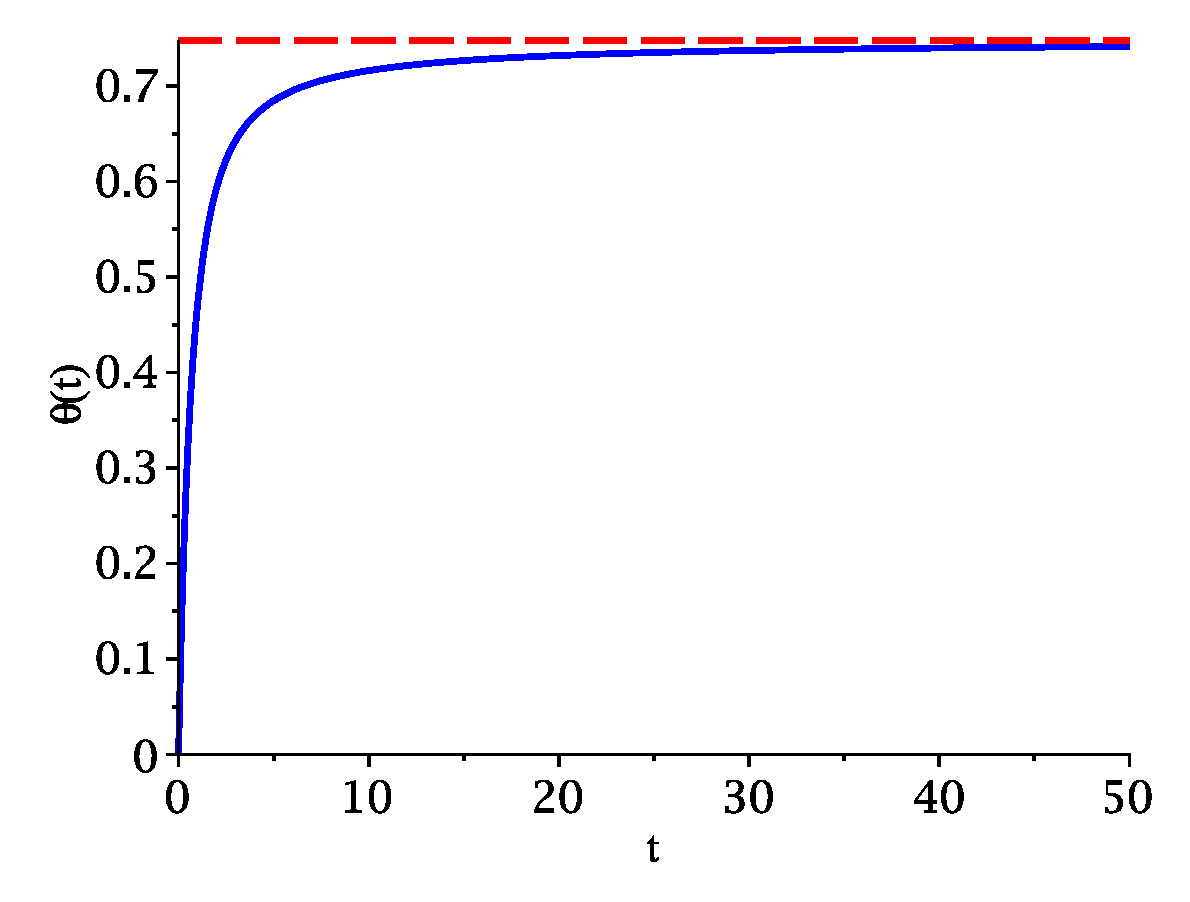
\includegraphics[scale = 0.35]{theta_01.eps}
%	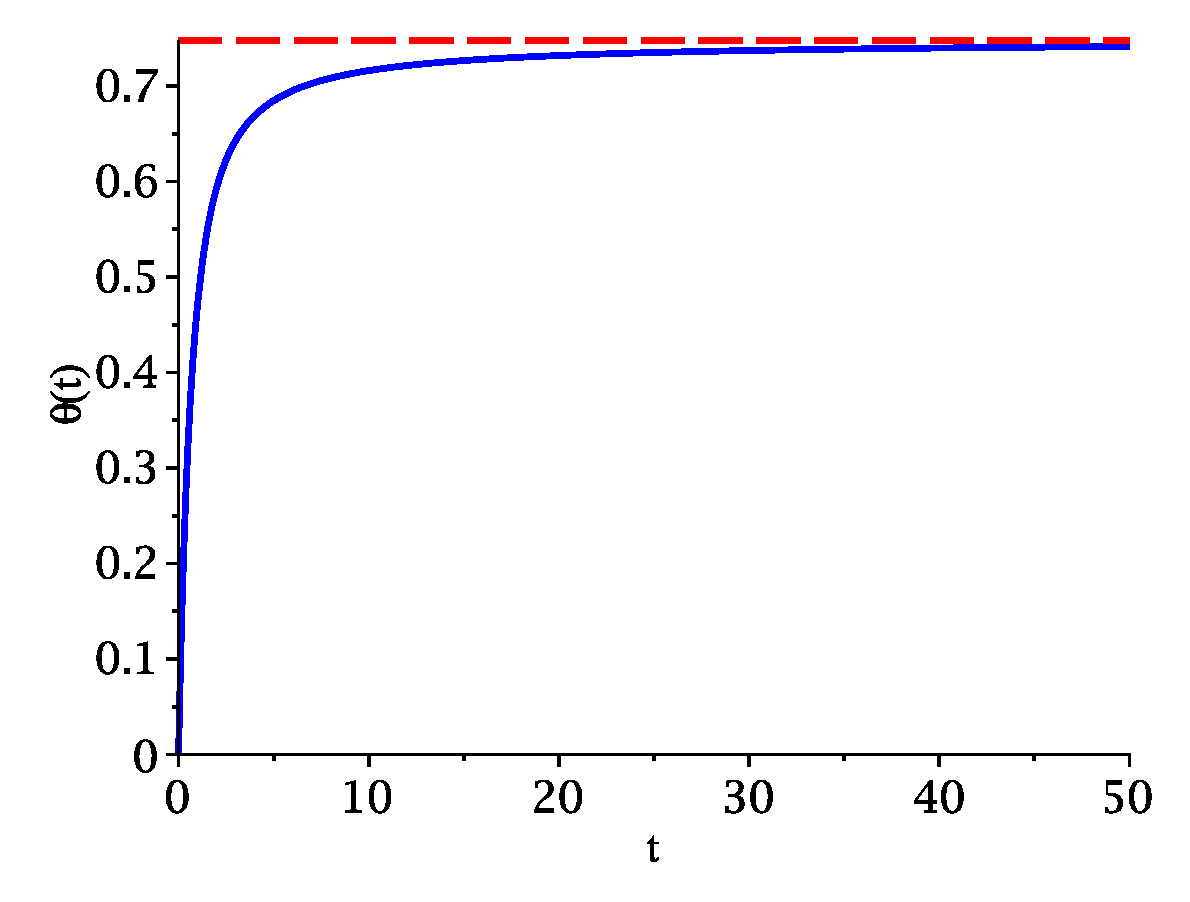
\includegraphics[width=\textwidth]{theta_01.eps}
	\caption{The coverage function}
	\label{fig:tcf1}
\end{figure}\medskip

We now look at the behaviour of the gap density function, $P(x, t)$, as a function of $x$ 
for different values of $t$. \bigskip

\begin{figure}[h!]
	\centering
%	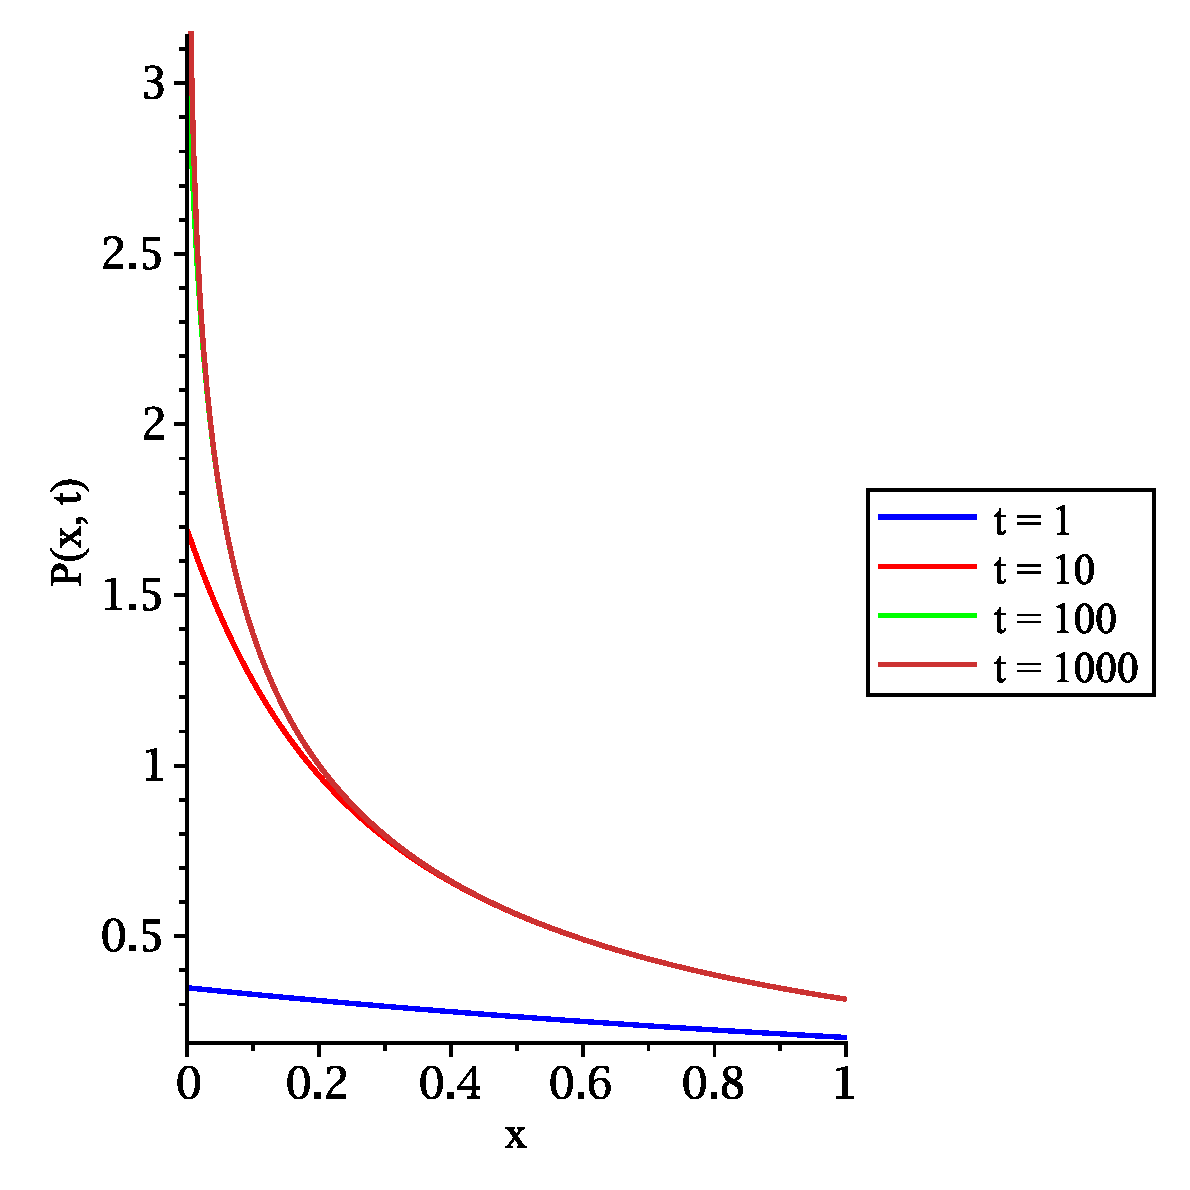
\includegraphics[scale = 0.35]{gap_density_01.eps}
	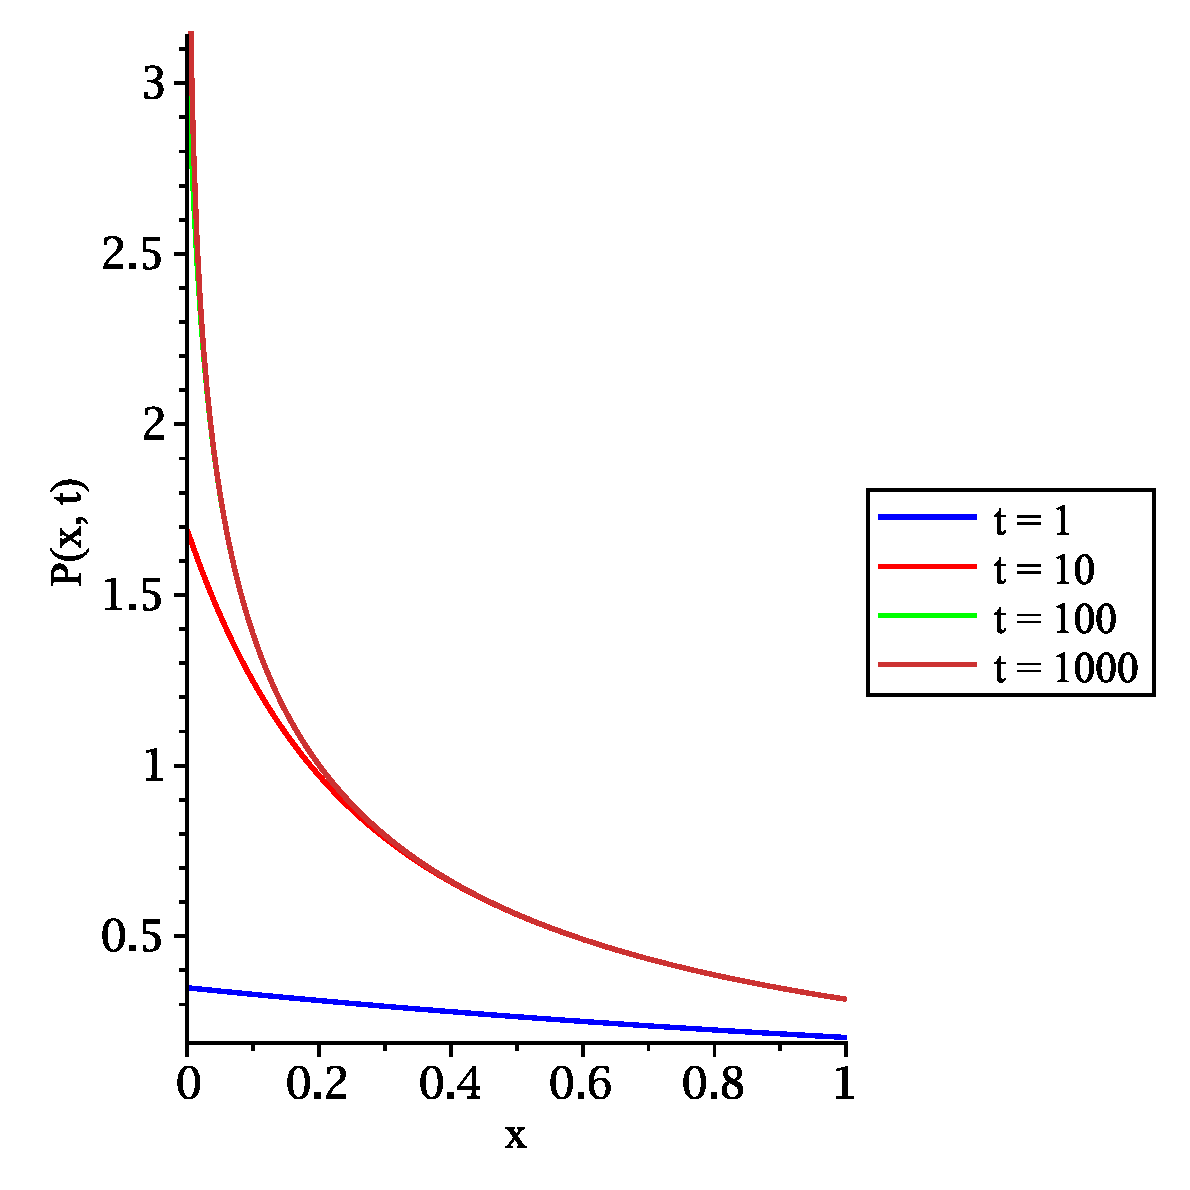
\includegraphics[width=\textwidth]{gap_density_01.eps}
	\caption{The gap density function for $x < 1$}
	\label{fig:gdf1}
\end{figure}\medskip

In figure \ref{fig:gdf1} we see the behaviour of the gap density function for $x < 1$ and 
for a range of values of $t$. As can be seen, as $t$ increases, the density of smaller gaps 
increases sharply, as is to be expected due to the increasing fragmentation, but the density 
of larger gaps within the range becomes more constant, again to be expected because these 
larger gaps are still less than the size of a car, so cannot be occupied, and hence remain 
unchanged. \bigskip

\begin{figure}[h!]
	\centering
%	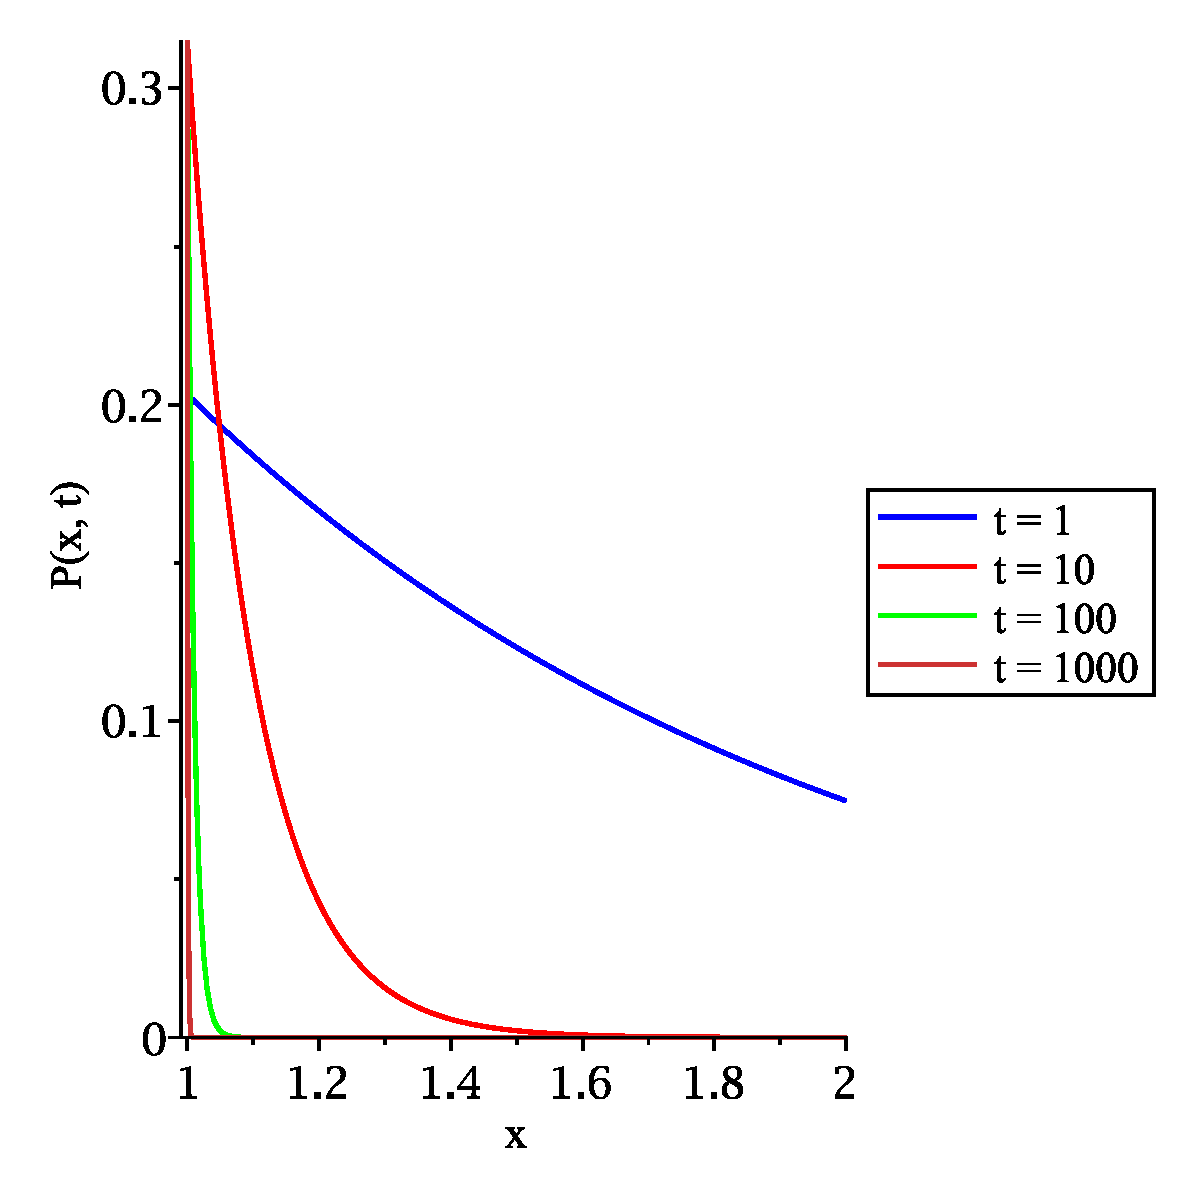
\includegraphics[scale = 0.35]{gap_density_02.eps}
	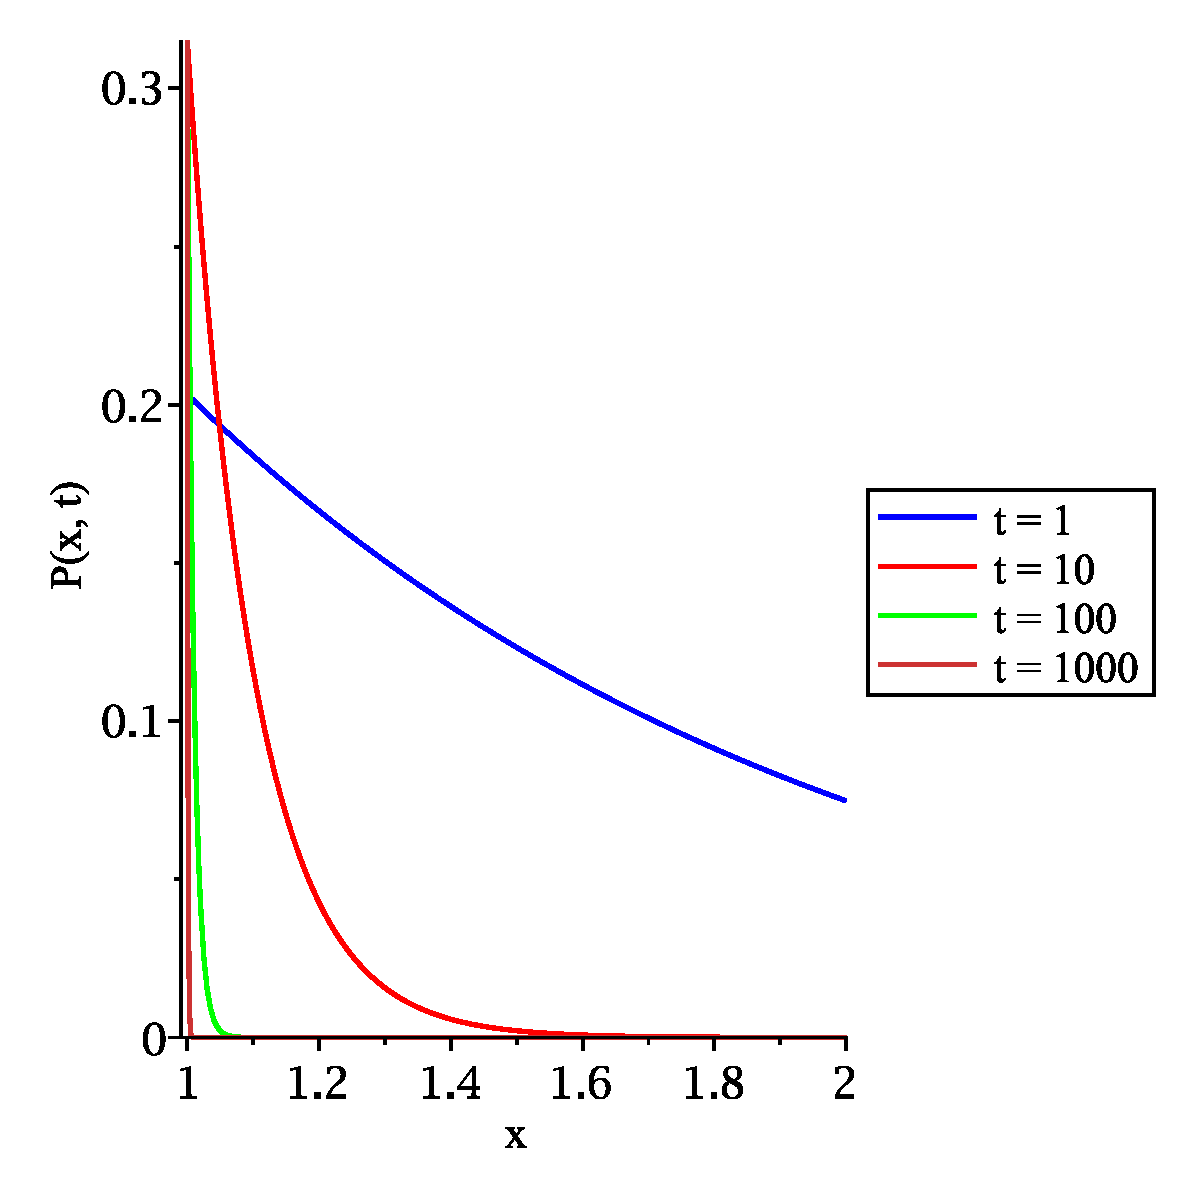
\includegraphics[width=\textwidth]{gap_density_02.eps}
	\caption{The gap density function for $x \geq 1$}
	\label{fig:gdf2}
\end{figure}\medskip

In figure \ref{fig:gdf2} we see the behaviour of the gap density function for $x \geq 1$ and 
for a range of values of $t$. As can be seen, as $t$ increases, the density of smaller gaps 
increases sharply, again as is to be expected due to the increasing fragmentation, but the 
density of larger gaps within the range reduces, again to be expected, because these larger 
gaps are destroyed by cars, and all that remain are gaps not large enough to accommodate cars. \bigskip

\newpage

We next look at the behaviour of the gap density function, $P(x, t)$, as a function of $t$ 
for different values of $x$. \bigskip

\begin{figure}[h!]
	\centering
	%	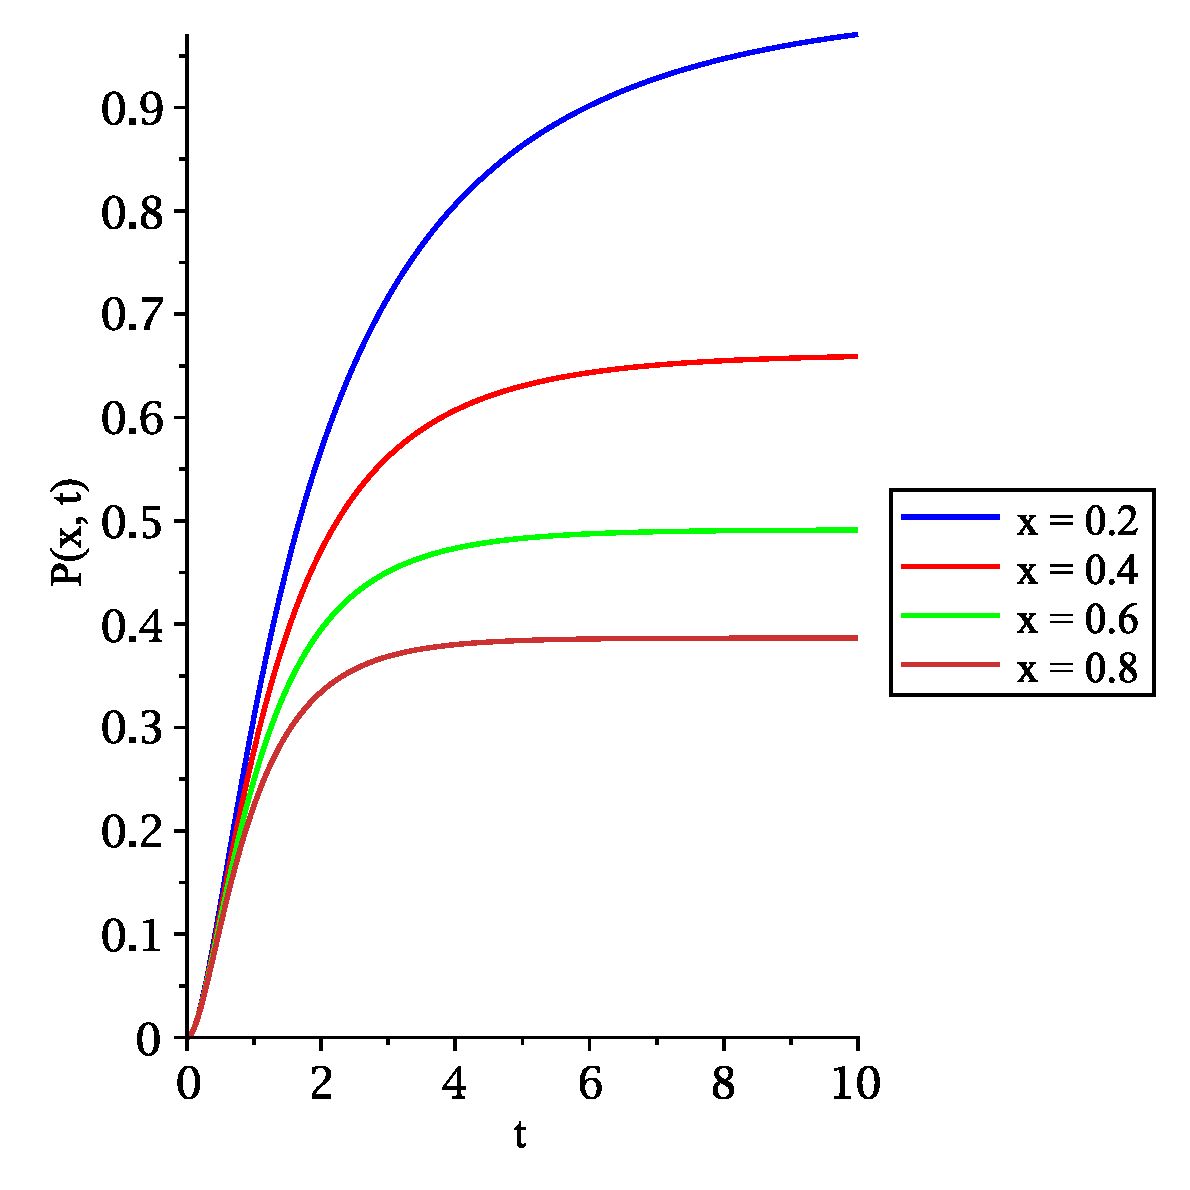
\includegraphics[scale = 0.35]{gap_density_03.eps}
	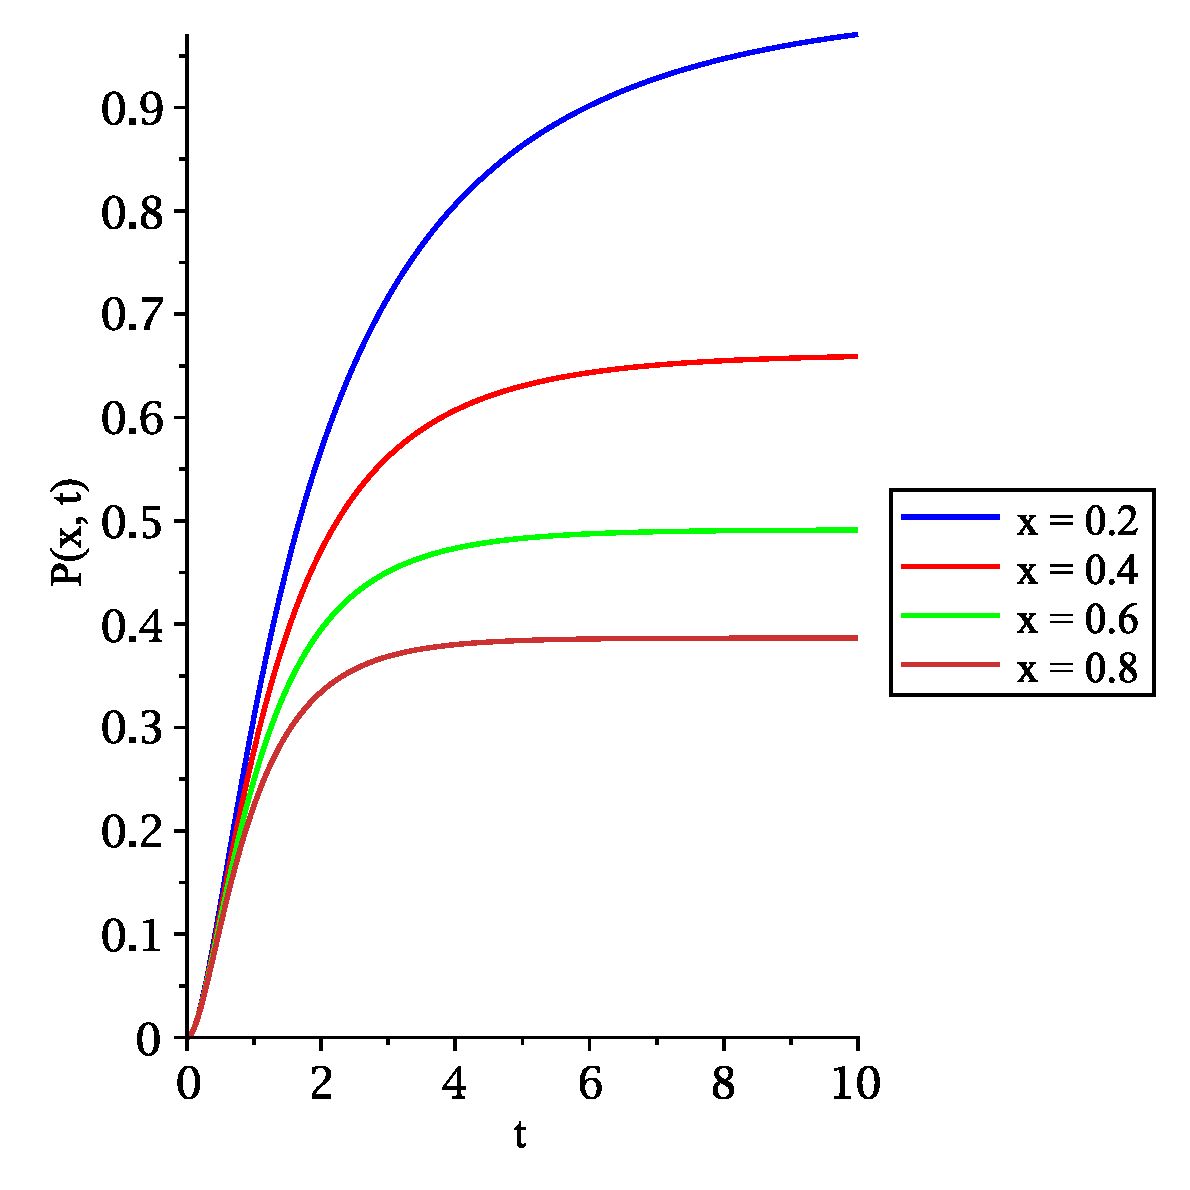
\includegraphics[width=\textwidth]{gap_density_03.eps}
	\caption{The gap density function}
	\label{fig:gdf3}
\end{figure}\medskip

In figure \ref{fig:gdf3} we see the behaviour of the gap density function for a range of 
values of $x < 1$. As can be seen, as $t$ increases, the density of these smaller gaps 
increases to a limit. This is to be expected due to the fact that as the parking process 
continues, eventually gaps, which are less than the size of a car, remain and can never 
be destroyed. \bigskip

\begin{figure}[h!]
	\centering
	%	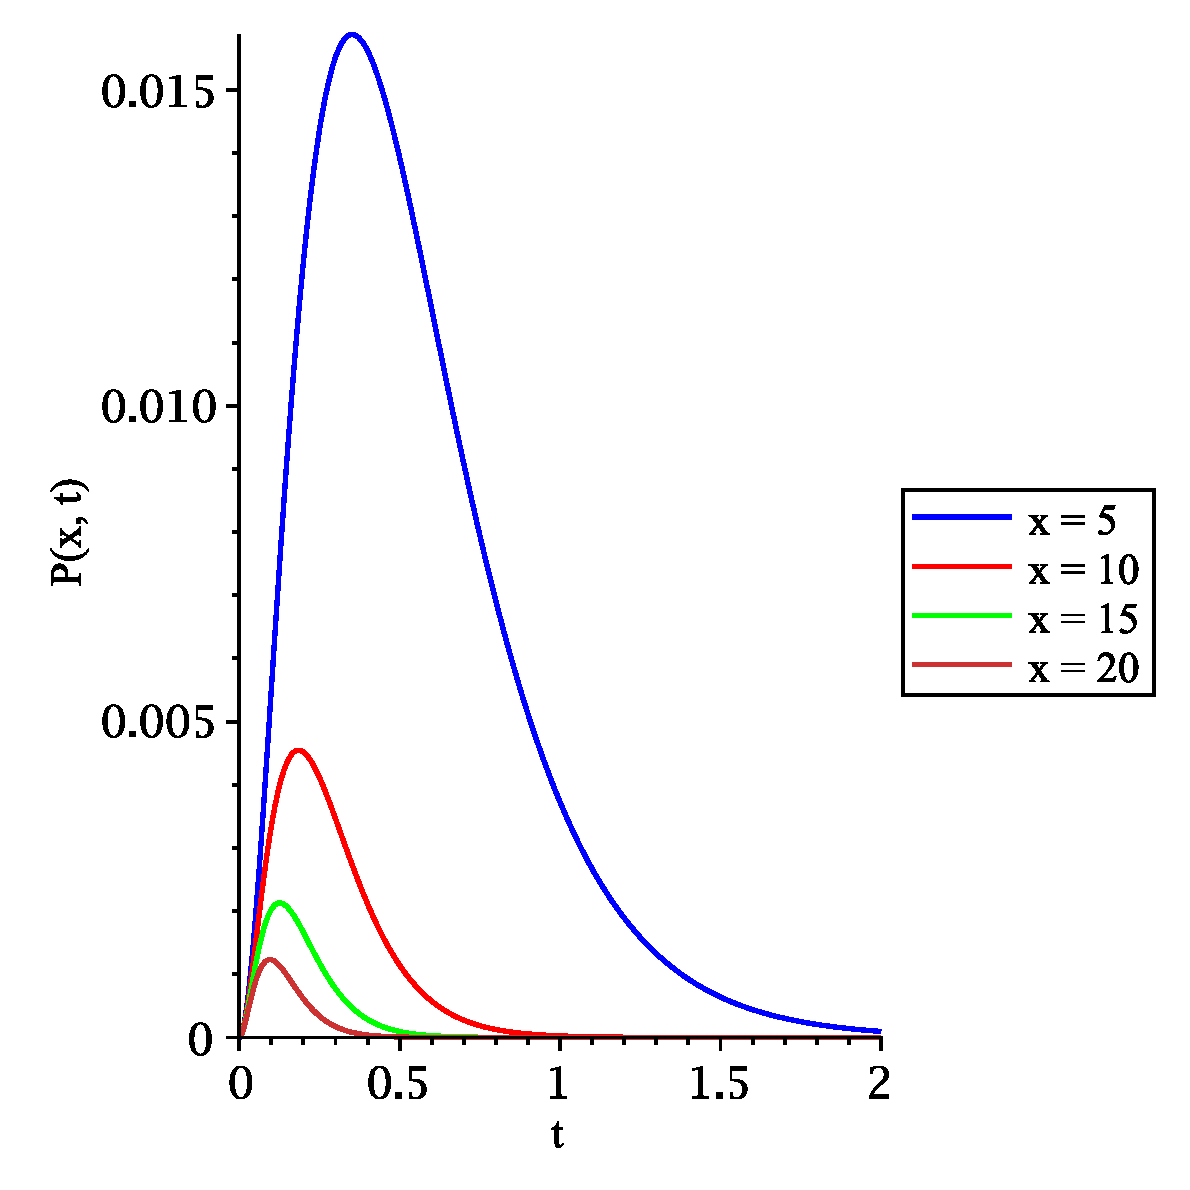
\includegraphics[scale = 0.35]{gap_density_04.eps}
	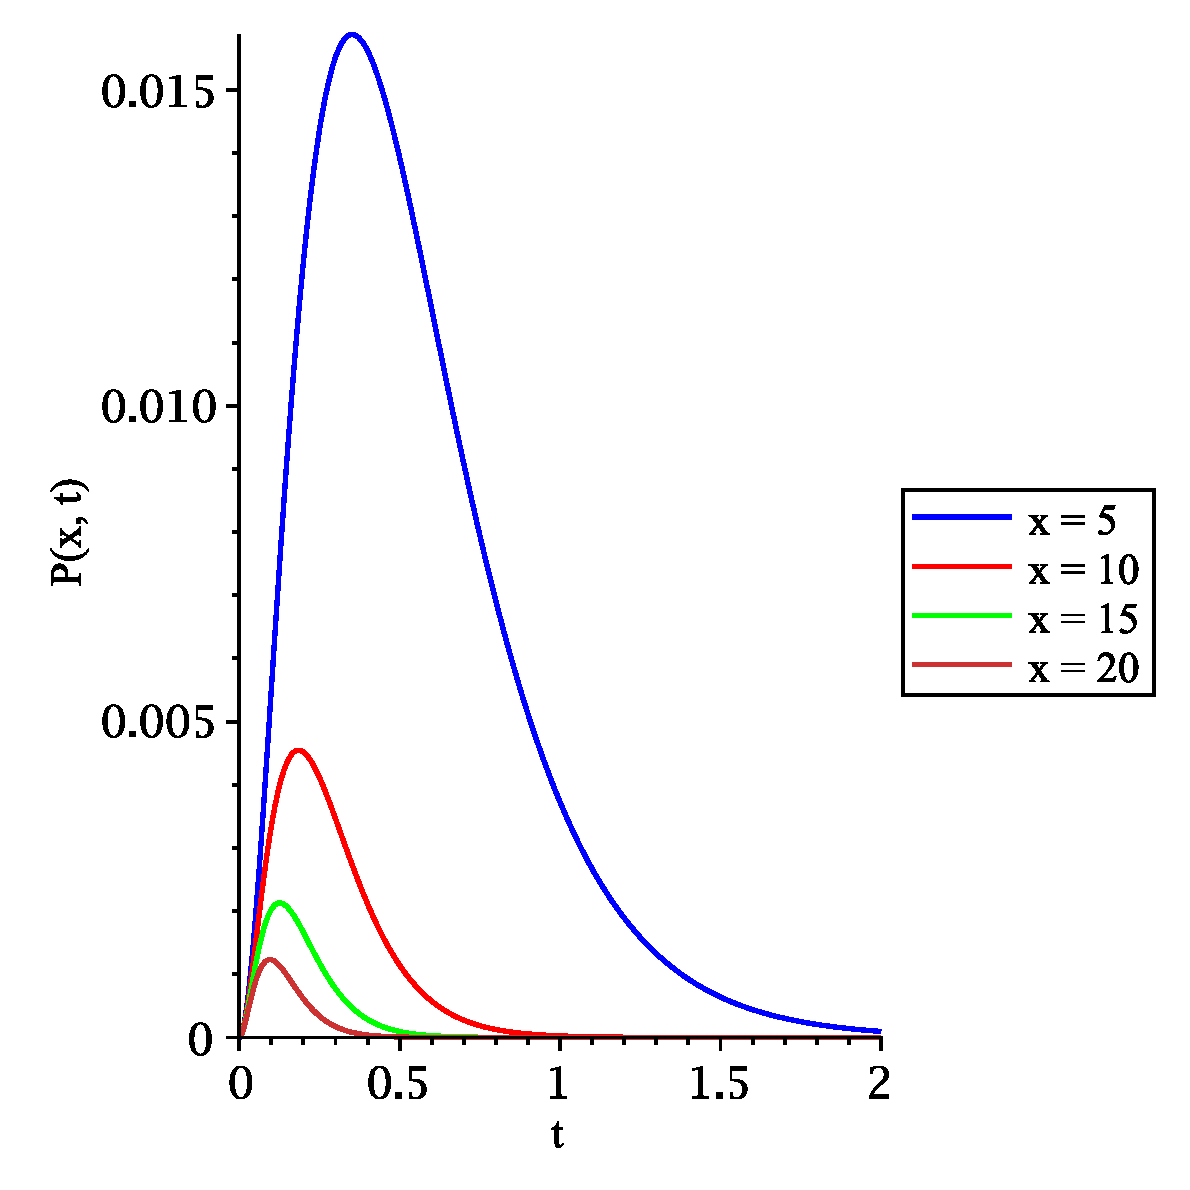
\includegraphics[width=\textwidth]{gap_density_04.eps}
	\caption{The gap density function}
	\label{fig:gdf4}
\end{figure}\medskip

In figure \ref{fig:gdf4} we see the behaviour of the gap density function for a range of 
values of $x \geq 1$. As can be seen, as $t$ increases, the density of these larger gaps 
increases sharply to a maximum, before decreasing, and approaching $0$. This is to be 
expected due to the fact that, as unit cars are initially parked they leave large gaps 
which are eventually destroyed in the parking process. \bigskip











\section{Remarks}

With the kinetic approach we have successfully modelled the process with respect to it's 
time evolution, rather than merely providing a means of evaluating $C_R$. This is a big 
step forward from the previous approaches. \bigskip

It should be noted that the approach of reducing the rate equation to an ODE breaks down 
for finite $L$: \bigskip

\begin{eqnarray*}
			\frac{\partial}{\partial t} (A(t) e^{-(x - 1)t}) & = & -(x - 1) A(t) e^{-(x - 1)t} + 2 \int_{x + 1}^{L} A(t) e^{-(y - 1)t} dy \\\\
	A^{\prime}(t) e^{-(x - 1)t} - (x - 1) A(t) e^{-(x - 1)t} & = & -(x - 1) A(t) e^{-(x - 1)t} + 2 A(t) \left. \frac{e^{-(y - 1)t}}{-t} \right|_{y = x + 1}^{L} \\\\
								 A^{\prime}(t) e^{-(x - 1)t} & = & 2 A(t) \left[ -\frac{e^{-t}}{t} e^{-(L - 2)t} + \frac{e^{-t}}{t} e^{-(x - 1)t} \right] \\\\
															 & = & 2 A(t) \frac{e^{-t}}{t} \left[ e^{-(x - 1)t} - e^{-(L - 2)t} \right]
\end{eqnarray*}\medskip

Hence finite $L$ prevents us from reducing the equation to a more manageable ODE, and it is clear 
that the imposition of $L \to \infty$ is made for mathematical reasons. \bigskip














\chapter{Generalizations}











\section{Parking with overlap}

We now look at the problem of parking with overlap, which is of practical 
interest in the context of particle adsorption (see \cite{roach2000parking}). 
Let $\phi$ denote the region of overlap, with $0 \leq \phi \leq 1$. We 
therefore have an exclusion zone around the centre of a car of length 
$1 - \phi$. Our problem is now the process of finding parking spots where 
exclusion zones do not overlap. This is equivalent to the parking problem 
but instead of dealing with cars of unit length we park the exclusion zones 
of length $1 - \phi$. We introduce a new gap density function 
$P_{\phi}(x, t)$ taking this into account, with allowed overlap $\phi$. \bigskip

Let $\bar{x}$ denote the distance between cars, and $x$ denote the distance 
between exclusion zones. Clearly $\bar{x} = x - \phi$. From this we can see 
that the distance between exclusion zones is always positive, but the distance 
between cars can be negative, in the case of overlap. \bigskip

Similar to the Kinetic approach, we define a rate equation for the creation and 
destruction of gaps for the overlap case: \bigskip

\begin{eqnarray*}
	\frac{\partial P_{\phi}(x, t)}{\partial t} = 
	\begin{dcases}
		2 \int_{x + 1 - \phi}^{\infty} P_{\phi}(y, t) dy                                   & \text{for } x < 1 - \phi \\\\
		-(x - 1 + \phi) P_{\phi}(x, t) + 2 \int_{x + 1 - \phi}^{\infty} P_{\phi}(y, t) dy  & \text{for } x \geq 1 - \phi
	\end{dcases}
\end{eqnarray*}\medskip

We take a similar approach to solving the above as was taken in the Kinetic 
approach. i.e. if we let: \bigskip

\[
	P_{\phi}(x, t) = A(t) e^{-(x - 1 + \phi)t}
\]\medskip 

and make the further substitution $A(t) = t^2 F_{\phi}(t)$, we find that: \bigskip

\[
	F_{\phi}(t) = \exp \left( -2 \int_{0}^{t} \frac{(1 - e^{-(1 - \phi)\tau})}{\tau} d\tau \right)
\]\medskip

The gap density function for gaps between exclusion zones becomes: \bigskip

\begin{eqnarray*}
	P_{\phi}(x, t) = 
	\begin{dcases}
		2 \int_{0}^{t} \tau F_{\phi}(\tau) e^{-x\tau} d\tau		& \text{for } x < 1 - \phi \\\\
		t^2 F_{\phi}(t) e^{-(x - 1 + \phi)t}					& \text{for } x \geq 1 - \phi 
	\end{dcases}
\end{eqnarray*}\medskip

and coverage by exclusion zone becomes: \bigskip

\begin{eqnarray*}
			\frac{d \theta_{\phi}}{dt} & = & (1 - \phi) F_{\phi}(t) \\\\
	 \therefore \quad \theta_{\phi}(t) & = & (1 - \phi) \int_{0}^{t} F_{\phi}(\tau) d\tau
\end{eqnarray*}\medskip

In figure \ref{fig:cfo1} we see the behaviour of the coverage function for 
different values of $\phi$. As is to be expected, the coverage tends towards 
$C_{R}$ as $t$ increases. \bigskip

\begin{figure}[h!]
	\centering
	%	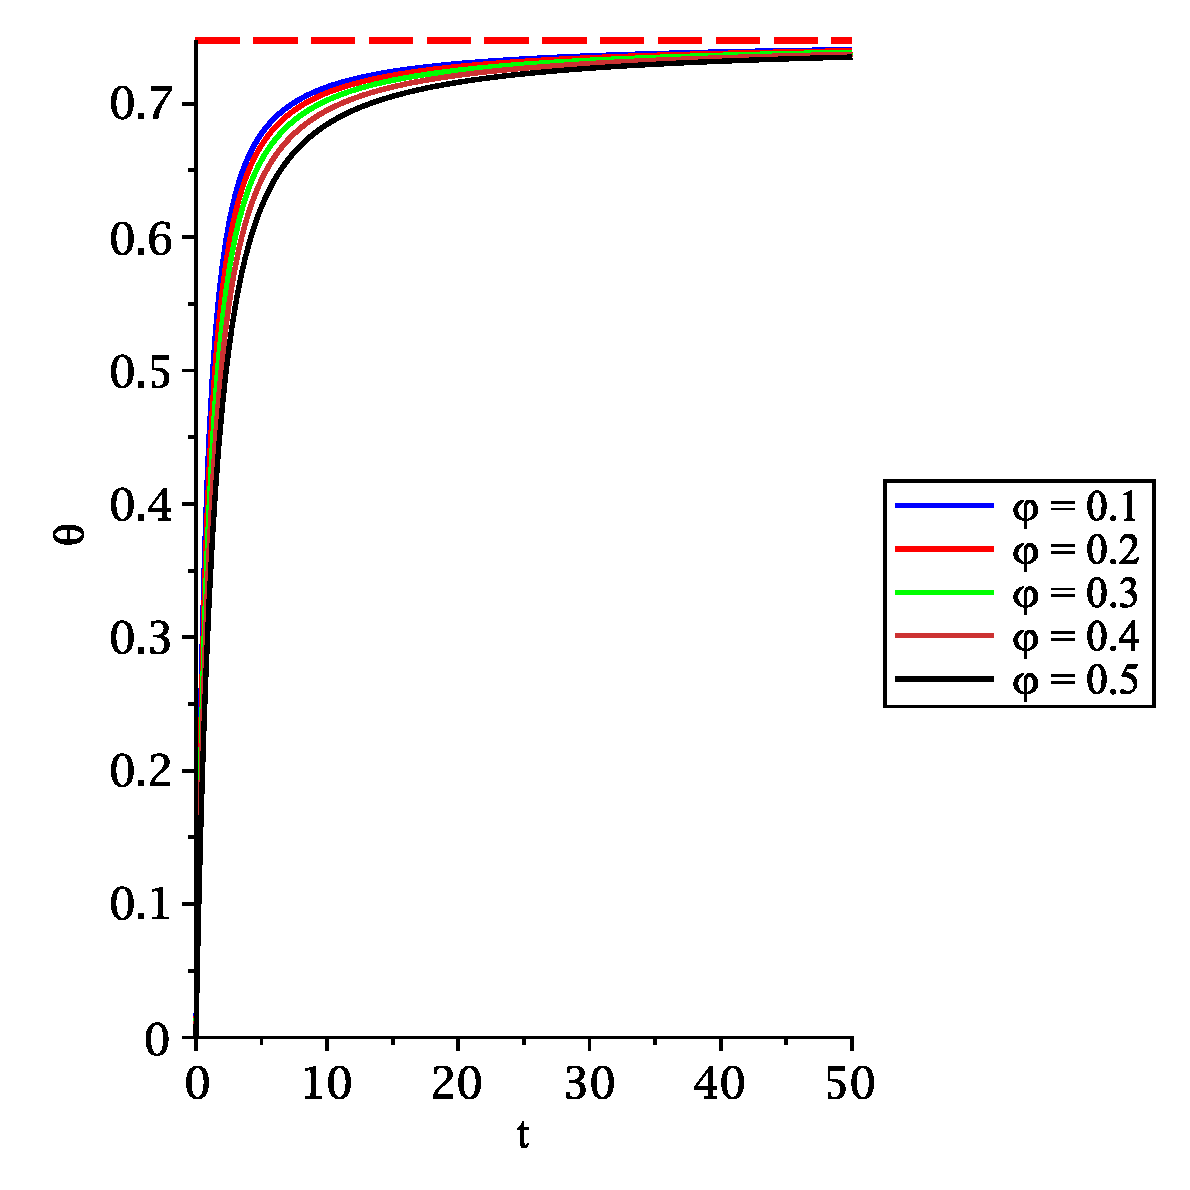
\includegraphics[scale = 0.35]{coverage_overlap_01.eps}
	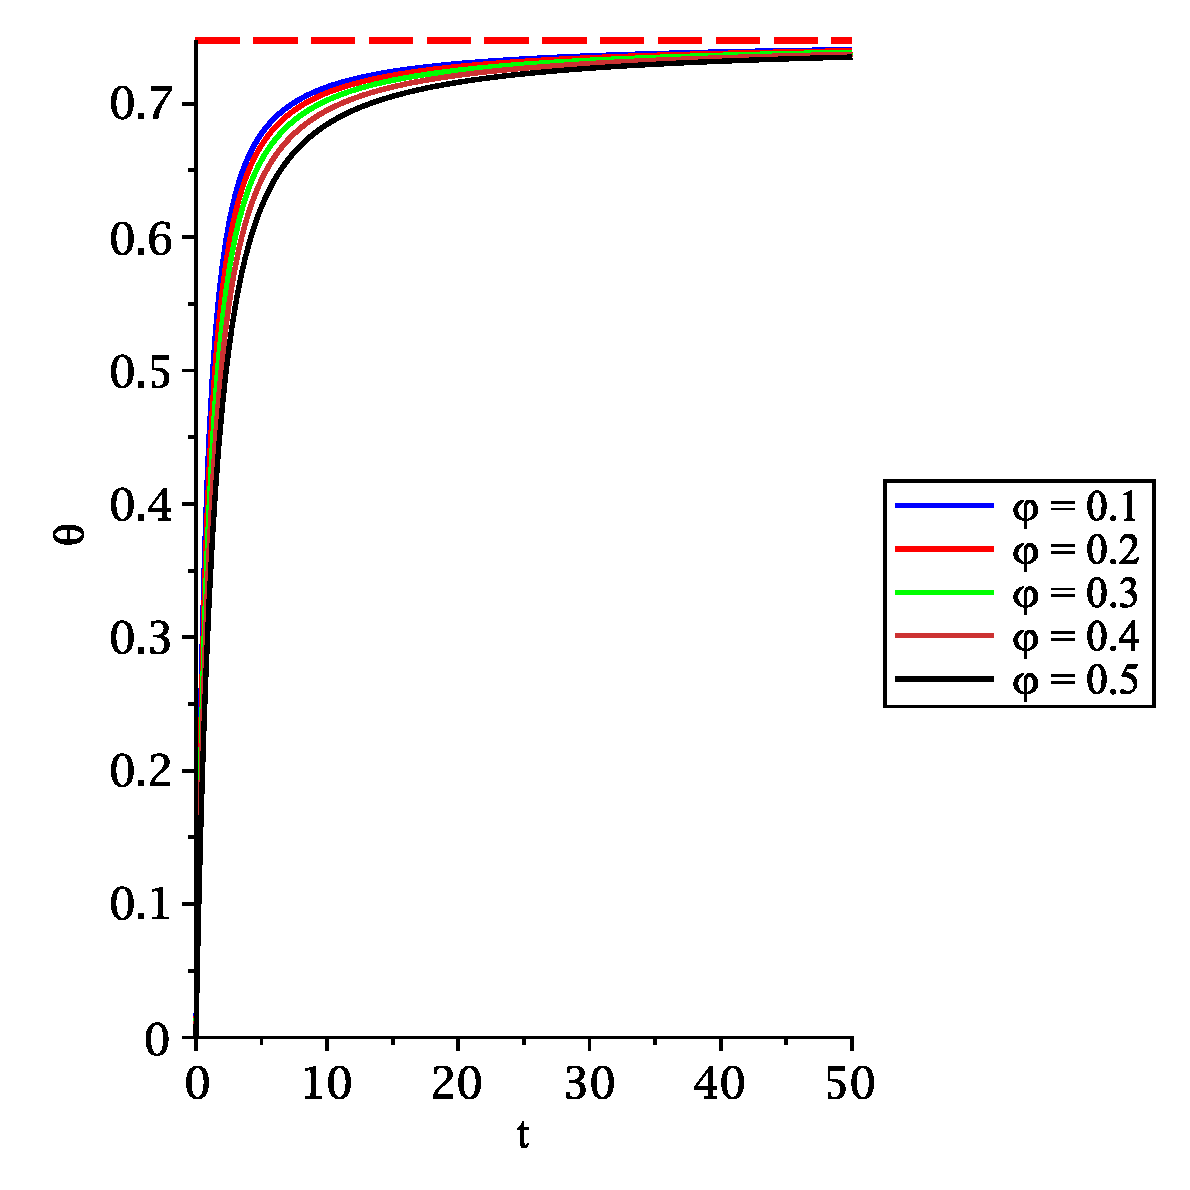
\includegraphics[width=\textwidth]{coverage_overlap_01.eps}
	\caption{The coverage function - overlap case}
	\label{fig:cfo1}
\end{figure}\medskip

The gap density function for gaps between cars, $\bar{x} = x - \phi$,  becomes: \bigskip

\begin{eqnarray*}
	Q_{\phi}(\bar{x}, t) = 
	\begin{dcases}
		2 \int_{0}^{t} \tau F_{\phi}(\tau) e^{-(\bar{x} + \phi)\tau} d\tau			& \text{for } \bar{x} < 1 - 2 \phi \\\\
		t^2 F_{\phi}(t) e^{-(\bar{x} - 1 + 2 \phi)t}								& \text{for } \bar{x} \geq 1 - 2 \phi 
	\end{dcases}
\end{eqnarray*}\medskip

and coverage by cars becomes: \bigskip

\[
	\Theta_{\phi}(t) = 1 - \int_{0}^{\infty} \bar{x} Q_{\phi}(\bar{x}, t) d\bar{x}
\]\medskip

Differentiating with respect to $t$ we get: \bigskip

\begin{eqnarray*}
	\frac{d \Theta_{\phi}}{dt} & = & -\frac{\partial}{\partial t} \int_{0}^{\infty} \bar{x} Q_{\phi}(\bar{x}, t) d\bar{x} \\\\
							   & = & -\frac{\partial}{\partial t} \left( \int_{0}^{1 - 2 \phi} \bar{x} Q_{\phi}(\bar{x}, t) d\bar{x} 
										- \int_{1 - 2 \phi}^{\infty} \bar{x} Q_{\phi}(\bar{x}, t) d\bar{x} \right) \\\\
							   & = & -\frac{\partial}{\partial t} \left( \int_{0}^{1 - 2 \phi} \bar{x} \left( 2 \int_{0}^{t} \tau F_{\phi}(\tau) e^{-(\bar{x} + \phi)\tau} d\tau \right) d\bar{x} 
										- \int_{1 - 2 \phi}^{\infty} \bar{x} t^2 F_{\phi}(t) e^{-(\bar{x} - 1 + 2 \phi)t} d\bar{x} \right) \\\\
							   & = & -\frac{\partial}{\partial t} \int_{0}^{1 - 2 \phi} \bar{x} \left( 2 \int_{0}^{t} \tau F_{\phi}(\tau) e^{-(\bar{x} + \phi)\tau} d\tau \right) d\bar{x} 
										- \frac{\partial}{\partial t} \int_{1 - 2 \phi}^{\infty} \bar{x} t^2 F_{\phi}(t) e^{-(\bar{x} - 1 + 2 \phi)t} d\bar{x} 
\end{eqnarray*}\medskip

for $\phi < \frac{1}{2}$. We will deal with each part of the right hand side separately. Starting with the first part: \bigskip

\begin{eqnarray*}
	-\frac{\partial}{\partial t} \int_{0}^{1 - 2 \phi} \bar{x} \left( 2 \int_{0}^{t} \tau F_{\phi}(\tau) e^{-(\bar{x} + \phi)\tau} d\tau \right) d\bar{x} & = & 
			-\int_{0}^{1 - 2 \phi} \bar{x} \left( 2 \frac{\partial}{\partial t} \int_{0}^{t} \tau F_{\phi}(\tau) e^{-(\bar{x} + \phi)\tau} d\tau \right) d\bar{x} \\\\
																																						  & = & 
			-\int_{0}^{1 - 2 \phi} \bar{x} 2 t F_{\phi}(t) e^{-(\bar{x} + \phi)t} d\bar{x} \\\\
																																						  & = & 
			-2 t F_{\phi}(t) e^{-\phi t} \int_{0}^{1 - 2 \phi} \bar{x} e^{-\bar{x} t} d\bar{x} \\\\
																																						  & = & 
			-2 t F_{\phi}(t) e^{-\phi t} \left[ - \frac{(1 - 2 \phi) e^{-(1 - 2 \phi)t}}{t} - \frac{e^{-(1 - 2 \phi)t}}{t^2} + \frac{1}{t^2} \right] \\\\
																																						  & = & 
			2 F_{\phi}(t) (1 - 2 \phi) e^{-(1 - \phi) t} + \frac{2 F_{\phi}(t) e^{-(1 - \phi)t}}{t} - \frac{2 F_{\phi}(t) e^{-\phi t}}{t}
\end{eqnarray*}\medskip

moving on to the second part: \bigskip

\begin{eqnarray*}
	-\frac{\partial}{\partial t} \int_{1 - 2 \phi}^{\infty} \bar{x} t^2 F_{\phi}(t) e^{-(\bar{x} - 1 + 2 \phi)t} d\bar{x} & = & 
			-\int_{1 - 2 \phi}^{\infty} \bar{x} \frac{\partial}{\partial t} \left( t^2 F_{\phi}(t) e^{-(\bar{x} - 1 + 2 \phi)t} \right) d\bar{x} \\\\
																														  & = & 
			-\int_{1 - 2 \phi}^{\infty} \bar{x} \frac{\partial}{\partial t} \left( t^2 F_{\phi}(t) e^{(1 - 2 \phi)t} e^{-\bar{x} t} \right) d\bar{x} 
\end{eqnarray*}\medskip

The differential within the integral is: \bigskip

\begin{eqnarray*}
	\frac{\partial}{\partial t} \left( t^2 F_{\phi}(t) e^{(1 - 2 \phi)t} e^{-\bar{x} t} \right) & = & 2 t F_{\phi}(t) e^{(1 - 2 \phi)t} e^{-\bar{x} t} \\\\
																								&   & + t^2 F_{\phi}^{\prime}(t) e^{(1 - 2 \phi)t} e^{-\bar{x} t} \\\\
																								&   & + t^2 F_{\phi}(t) (1 - 2 \phi) e^{(1 - 2 \phi)t} e^{-\bar{x} t} \\\\
																								&   & - t^2 F_{\phi}(t) e^{(1 - 2 \phi)t} \bar{x} e^{-\bar{x} t} 
\end{eqnarray*}\medskip

so our integral becomes: \bigskip

\begin{eqnarray*}
	-\int_{1 - 2 \phi}^{\infty} \bar{x} \frac{\partial}{\partial t} \left( t^2 F_{\phi}(t) e^{(1 - 2 \phi)t} e^{-\bar{x} t} \right) d\bar{x} & = & 
			-\int_{1 - 2 \phi}^{\infty} \bar{x} 2 t F_{\phi}(t) e^{(1 - 2 \phi)t} e^{-\bar{x} t} d\bar{x} \\\\
																																			 &   & 
			- \int_{1 - 2 \phi}^{\infty} \bar{x} t^2 F_{\phi}^{\prime}(t) e^{(1 - 2 \phi)t} e^{-\bar{x} t} d\bar{x} \\\\
																																			 &   & 
			- \int_{1 - 2 \phi}^{\infty} \bar{x} t^2 F_{\phi}(t) (1 - 2 \phi) e^{(1 - 2 \phi)t} e^{-\bar{x} t} d\bar{x} \\\\
																																			 &   & 
			+ \int_{1 - 2 \phi}^{\infty} \bar{x} t^2 F_{\phi}(t) e^{(1 - 2 \phi)t} \bar{x} e^{-\bar{x} t} d\bar{x}
\end{eqnarray*}\medskip

taking each integral separately: \bigskip

\begin{eqnarray*}
	-\int_{1 - 2 \phi}^{\infty} \bar{x} 2 t F_{\phi}(t) e^{(1 - 2 \phi)t} e^{-\bar{x} t} d\bar{x} & = & -\int_{1 - 2 \phi}^{\infty} 2 t F_{\phi}(t) e^{(1 - 2 \phi)t} \bar{x} e^{-\bar{x} t} d\bar{x} \\\\
																								  & = & -2 t F_{\phi}(t) e^{(1 - 2 \phi)t} \int_{1 - 2 \phi}^{\infty} \bar{x} e^{-\bar{x} t} d\bar{x} \\\\
																								  & = & -2 t F_{\phi}(t) e^{(1 - 2 \phi)t} \left[ \frac{(1 - 2 \phi) e^{-(1 - 2 \phi)t}}{t} + \frac{e^{-(1 - 2 \phi)t}}{t^2} \right] \\\\
																								  & = & -2 t F_{\phi}(t) (1 - 2 \phi) - \frac{2 F_{\phi}(t)}{t}
\end{eqnarray*}\medskip

followed by: \bigskip

\begin{eqnarray*}
	-\int_{1 - 2 \phi}^{\infty} \bar{x} t^2 F_{\phi}^{\prime}(t) e^{(1 - 2 \phi)t} e^{-\bar{x} t} d\bar{x} & = & -\int_{1 - 2 \phi}^{\infty} t^2 F_{\phi}^{\prime}(t) e^{(1 - 2 \phi)t} \bar{x} e^{-\bar{x} t} d\bar{x} \\\\
																										   & = & -t^2 F_{\phi}^{\prime}(t) e^{(1 - 2 \phi)t} \int_{1 - 2 \phi}^{\infty} \bar{x} e^{-\bar{x} t} d\bar{x} \\\\
																										   & = & -t^2 F_{\phi}^{\prime}(t) e^{(1 - 2 \phi)t} \left[ \frac{(1 - 2 \phi) e^{-(1 - 2 \phi)t}}{t} + \frac{e^{-(1 - 2 \phi)t}}{t^2} \right] \\\\
																										   & = & -t F_{\phi}^{\prime}(t) (1 - 2 \phi) - F_{\phi}^{\prime} \\\\
																										   & = & -t F_{\phi}(t) \left( -2 \frac{(1 - e^{-(1 - \phi)t})}{t} \right) (1 - 2 \phi) - F_{\phi}(t) \left( -2 \frac{(1 - e^{-(1 - \phi)t})}{t} \right) \\\\
																										   & = & 2 F_{\phi}(t) (1 - 2 \phi) - 2 F_{\phi}(t) (1 - 2 \phi) e^{-(1 - \phi)t} + \frac{2 F_{\phi}(t)}{t} - \frac{2 F_{\phi}(t) e^{-(1 - \phi)t}}{t}
\end{eqnarray*}\medskip

here we make use of the fact that: \bigskip

\begin{eqnarray*}
							  F_{\phi}(t) & = & \exp \left( -2 \int_{0}^{t} \frac{(1 - e^{-(1 - \phi)\tau})}{\tau} d\tau \right) \\\\
	\therefore \quad F_{\phi}^{\prime}(t) & = & F_{\phi}(t) \left( -2 \frac{(1 - e^{-(1 - \phi)t})}{t} \right)
\end{eqnarray*}\medskip

followed by: \bigskip

\begin{eqnarray*}
	-\int_{1 - 2 \phi}^{\infty} \bar{x} t^2 F_{\phi}(t) (1 - 2 \phi) e^{(1 - 2 \phi)t} e^{-\bar{x} t} d\bar{x} & = & -\int_{1 - 2 \phi}^{\infty} t^2 F_{\phi}(t) (1 - 2 \phi) e^{(1 - 2 \phi)t} \bar{x} e^{-\bar{x} t} d\bar{x} \\\\
																											   & = & -t^2 F_{\phi}(t) (1 - 2 \phi) e^{(1 - 2 \phi)t} \int_{1 - 2 \phi}^{\infty} \bar{x} e^{-\bar{x} t} d\bar{x} \\\\
																											   & = & -t^2 F_{\phi}(t) (1 - 2 \phi) e^{(1 - 2 \phi)t} \left[ \frac{(1 - 2 \phi) e^{-(1 - 2 \phi)t}}{t} + \frac{e^{-(1 - 2 \phi)t}}{t^2} \right] \\\\
																											   & = & -t F_{\phi}(t) (1 - 2 \phi)^2 - F_{\phi}(t) (1 - 2 \phi)
\end{eqnarray*}\medskip

and finally: \bigskip

\begin{eqnarray*}
	\int_{1 - 2 \phi}^{\infty} \bar{x} t^2 F_{\phi}(t) e^{(1 - 2 \phi)t} \bar{x} e^{-\bar{x} t} d\bar{x} & = & \int_{1 - 2 \phi}^{\infty} t^2 F_{\phi}(t) e^{(1 - 2 \phi)t} \bar{x}^2 e^{-\bar{x} t} d\bar{x} \\\\
																										 & = & t^2 F_{\phi}(t) e^{(1 - 2 \phi)t} \int_{1 - 2 \phi}^{\infty} \bar{x}^2 e^{-\bar{x} t} d\bar{x} \\\\
																										 & = & t^2 F_{\phi}(t) e^{(1 - 2 \phi)t} \left[ \frac{(1 - 2 \phi)^2 e^{-(1 - 2 \phi)t}}{t} + \frac{2 (1 - 2 \phi) e^{-(1 - 2 \phi)t}}{t^2} + \frac{2 e^{-(1 - 2 \phi)t}}{t^3} \right] \\\\
																										 & = & t F_{\phi}(t) (1 - 2 \phi)^2 + 2 F_{\phi}(t) (1 - 2 \phi) + \frac{2 F_{\phi}(t)}{t} 
\end{eqnarray*}\medskip

combining all of the above we get: \bigskip

\begin{eqnarray*}
	\frac{d \Theta_{\phi}}{dt} & = & 2 F_{\phi}(t) (1 - 2 \phi) e^{-(1 - \phi) t} + \frac{2 F_{\phi}(t) e^{-(1 - \phi)t}}{t} - \frac{2 F_{\phi}(t) e^{-\phi t}}{t} \\\\
							   &   & - 2 t F_{\phi}(t) (1 - 2 \phi) - \frac{2 F_{\phi}(t)}{t} \\\\
							   &   & + 2 F_{\phi}(t) (1 - 2 \phi) - 2 F_{\phi}(t) (1 - 2 \phi) e^{-(1 - \phi)t} + \frac{2 F_{\phi}(t)}{t} - \frac{2 F_{\phi}(t) e^{-(1 - \phi)t}}{t} \\\\
							   &   & - t F_{\phi}(t) (1 - 2 \phi)^2 - F_{\phi}(t) (1 - 2 \phi) \\\\
							   &   & + t F_{\phi}(t) (1 - 2 \phi)^2 + 2 F_{\phi}(t) (1 - 2 \phi) + \frac{2 F_{\phi}(t)}{t} 
\end{eqnarray*}\medskip

after much cancellation, we are left with: \bigskip

\begin{eqnarray*}
	\frac{d \Theta_{\phi}}{dt} & = & \frac{2 F_{\phi}(t)}{t} - \frac{2 F_{\phi}(t) e^{-\phi t}}{t} + F_{\phi}(t) (1 - 2 \phi) \\\\
							   & = & F_{\phi}(t) \left[ \frac{2}{t} (1 - e^{-\phi t}) + 1 - 2 \phi \right]
\end{eqnarray*}\medskip

and hence: \bigskip

\[
	\Theta_{\phi} (t) = (1 - 2 \phi) \int_{0}^{t} F_{\phi}(\tau) d \tau  + \int_{0}^{t} F_{\phi}(\tau) \frac{2}{\tau} (1 - e^{-\phi \tau}) d \tau
\]\medskip

for $\phi < \frac{1}{2}$. Now similarly for the case when $\phi \geq \frac{1}{2}$: \bigskip

\begin{eqnarray*}
			\frac{d \Theta_{\phi}}{dt} & = & -\frac{\partial}{\partial t} \int_{0}^{\infty} \bar{x} Q_{\phi}(\bar{x}, t) d\bar{x} \\\\
									   & = & -\int_{0}^{\infty} \bar{x} \frac{\partial}{\partial t} \left( t^2 F_{\phi}(t) e^{(1 - 2 \phi)t} e^{-\bar{x} t} \right) d\bar{x} \\\\
									   & = & -2 t F_{\phi}(t) e^{(1 - 2 \phi)t} \int_{0}^{\infty} \bar{x} e^{-\bar{x} t} d\bar{x} \\\\
									   &   & - t^2 F_{\phi}^{\prime}(t) e^{(1 - 2 \phi)t} \int_{0}^{\infty} \bar{x} e^{-\bar{x} t} d\bar{x} \\\\
									   &   & - t^2 F_{\phi}(t) (1 - 2 \phi) e^{(1 - 2 \phi)t} \int_{0}^{\infty} \bar{x} e^{-\bar{x} t} d\bar{x} \\\\
									   &   & + t^2 F_{\phi}(t) e^{(1 - 2 \phi)t} \int_{0}^{\infty} \bar{x}^2 e^{-\bar{x} t} d\bar{x} \\\\
									   & = & -\frac{2}{t} F_{\phi}(t) e^{(1 - 2 \phi)t} - F_{\phi}^{\prime}(t) e^{(1 - 2 \phi)t} - F_{\phi}(t) (1 - 2 \phi) e^{(1 - 2 \phi)t} + \frac{2}{t} F_{\phi}(t) e^{(1 - 2 \phi)t} \\\\
									   & = & -F_{\phi}^{\prime}(t) e^{(1 - 2 \phi)t} - F_{\phi}(t) (1 - 2 \phi) e^{(1 - 2 \phi)t} \\\\
									   & = & -\frac{d}{dt} \left( F_{\phi}(t) e^{(1 - 2 \phi)t} \right) \\\\
	\therefore \quad \Theta_{\phi} (t) & = & -F_{\phi}(t) e^{(1 - 2 \phi)t} + C
\end{eqnarray*}\medskip

at $t = 0$ the coverage is $0$, and hence $C = 1$, giving us: \bigskip

\[
	\Theta_{\phi} (t) = 1 - F_{\phi}(t) e^{(1 - 2 \phi)t}
\]\medskip

so our coverage for cars is: \bigskip

\begin{eqnarray*}
	\Theta_{\phi}(t) = 
	\begin{dcases}
		(1 - 2 \phi) \int_{0}^{t} F_{\phi}(\tau) d \tau  + \int_{0}^{t} F_{\phi}(\tau) \frac{2}{\tau} (1 - e^{-\phi \tau}) d \tau			& \text{for } \phi < \frac{1}{2} \\\\
		1 - F_{\phi}(t) e^{(1 - 2 \phi)t}																									& \text{for } \phi \geq \frac{1}{2} 
	\end{dcases}
\end{eqnarray*}\medskip

\newpage

In figure \ref{fig:cp1} we see the behaviour of the coverage for cars for 
values of $\phi$ between $0$ and $0.5$. As is to be expected, the limit 
for each value of $\phi$ increases as $t$ increases. \bigskip

\begin{figure}[h!]
	\centering
	%	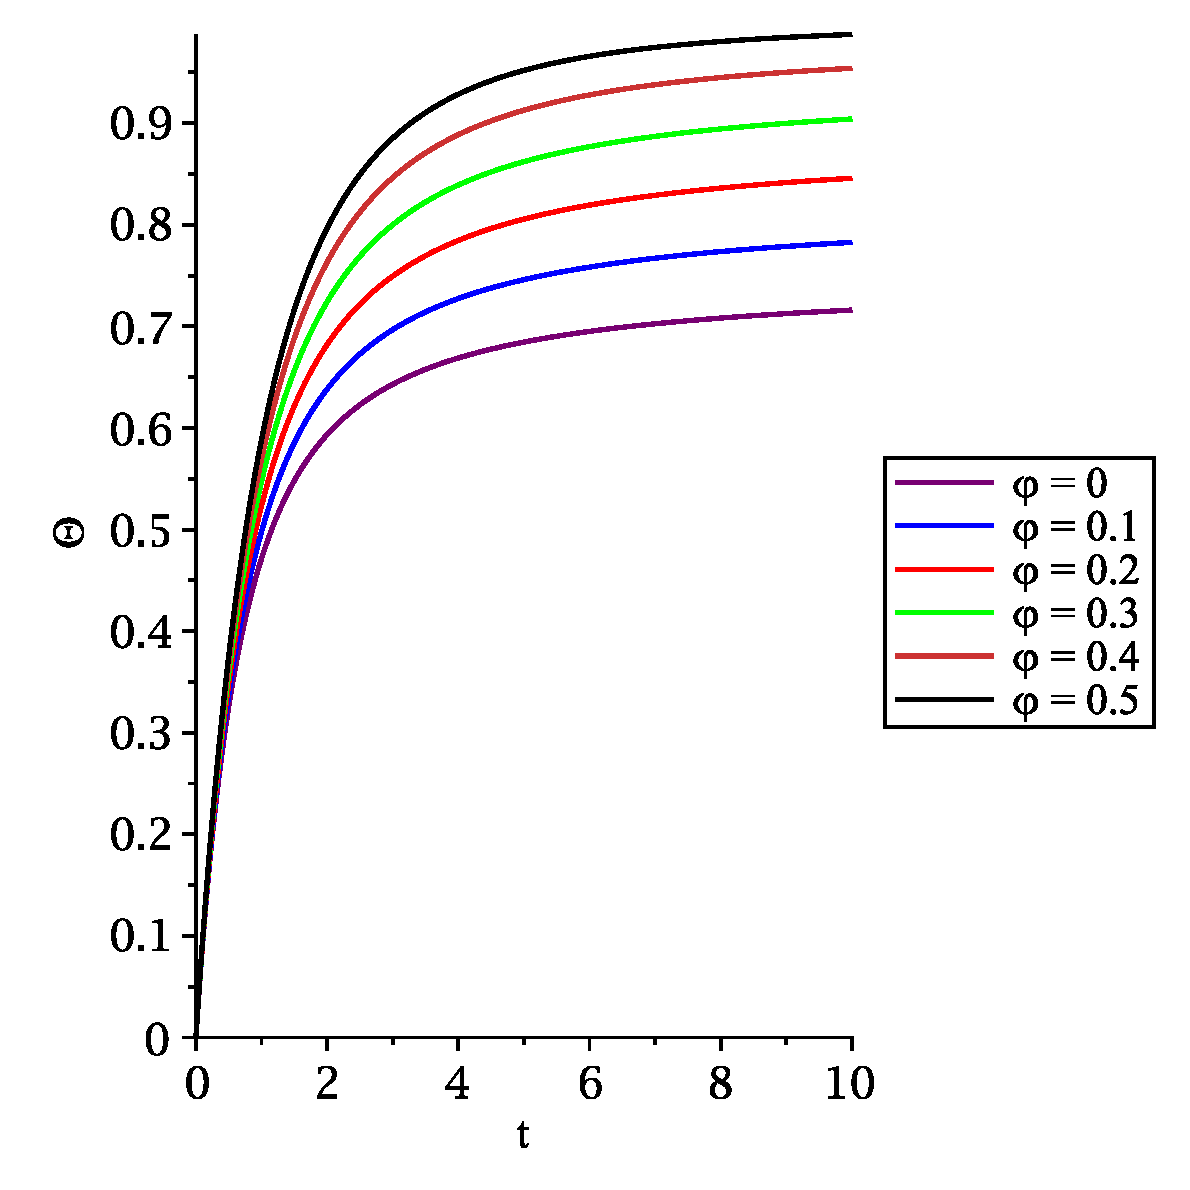
\includegraphics[scale = 0.35]{coverage_phi_01.eps}
	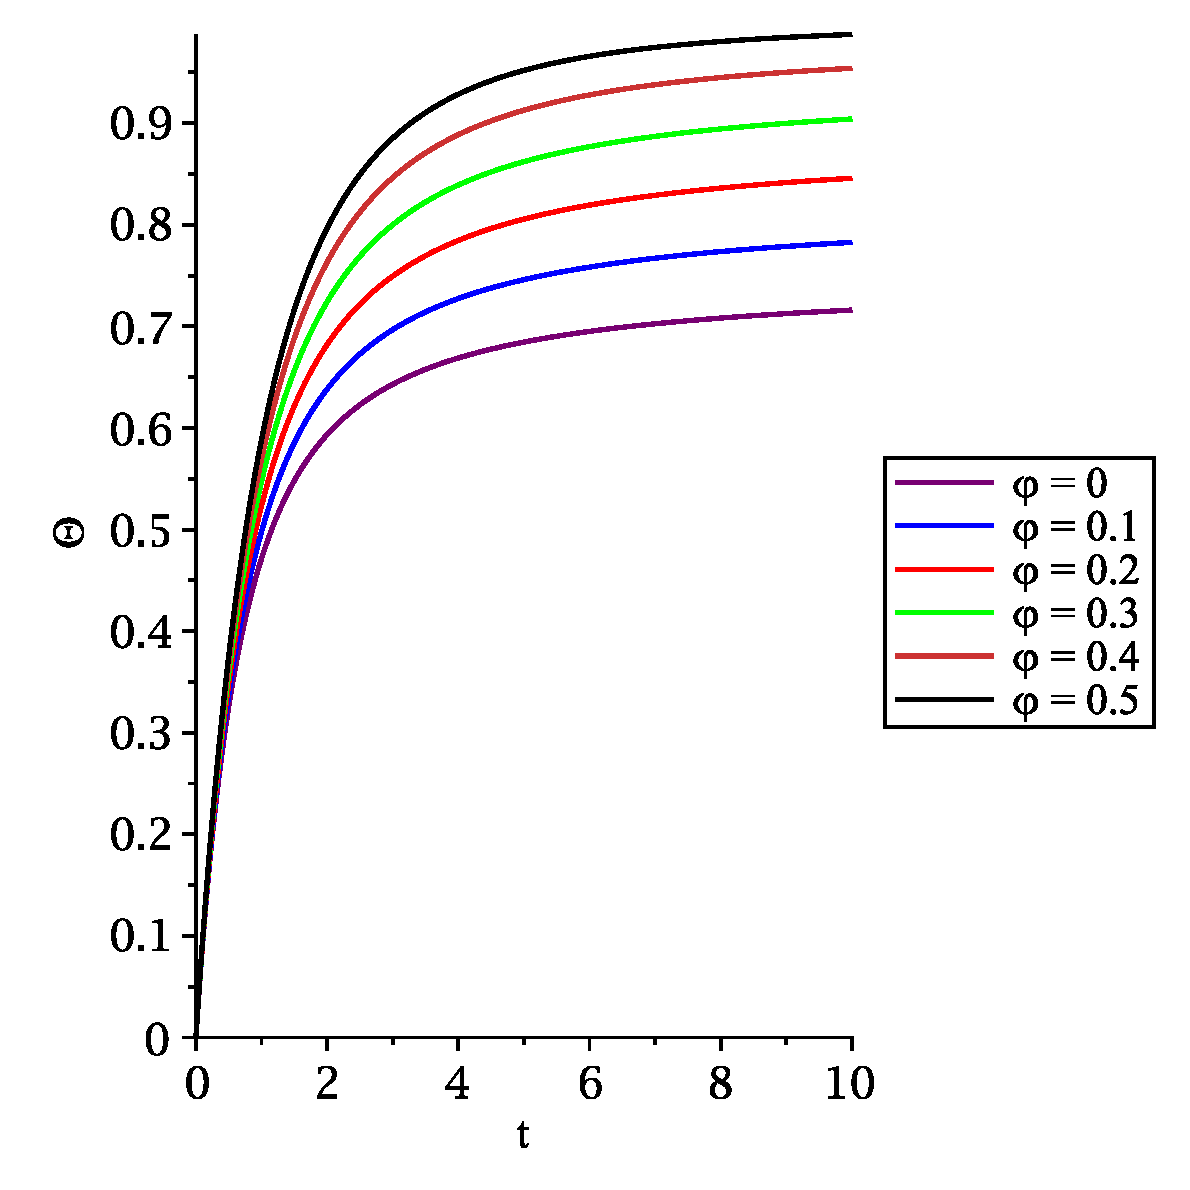
\includegraphics[width=\textwidth]{coverage_phi_01.eps}
	\caption{The coverage by cars}
	\label{fig:cp1}
\end{figure}\medskip

\newpage

In figure \ref{fig:cp2} we see the behaviour of the coverage for cars for 
values of $\phi$ between $0.5$ and $1$. As is to be expected, the coverage 
tends towards $1$ as $t$ increases. \bigskip

\begin{figure}[h!]
	\centering
	%	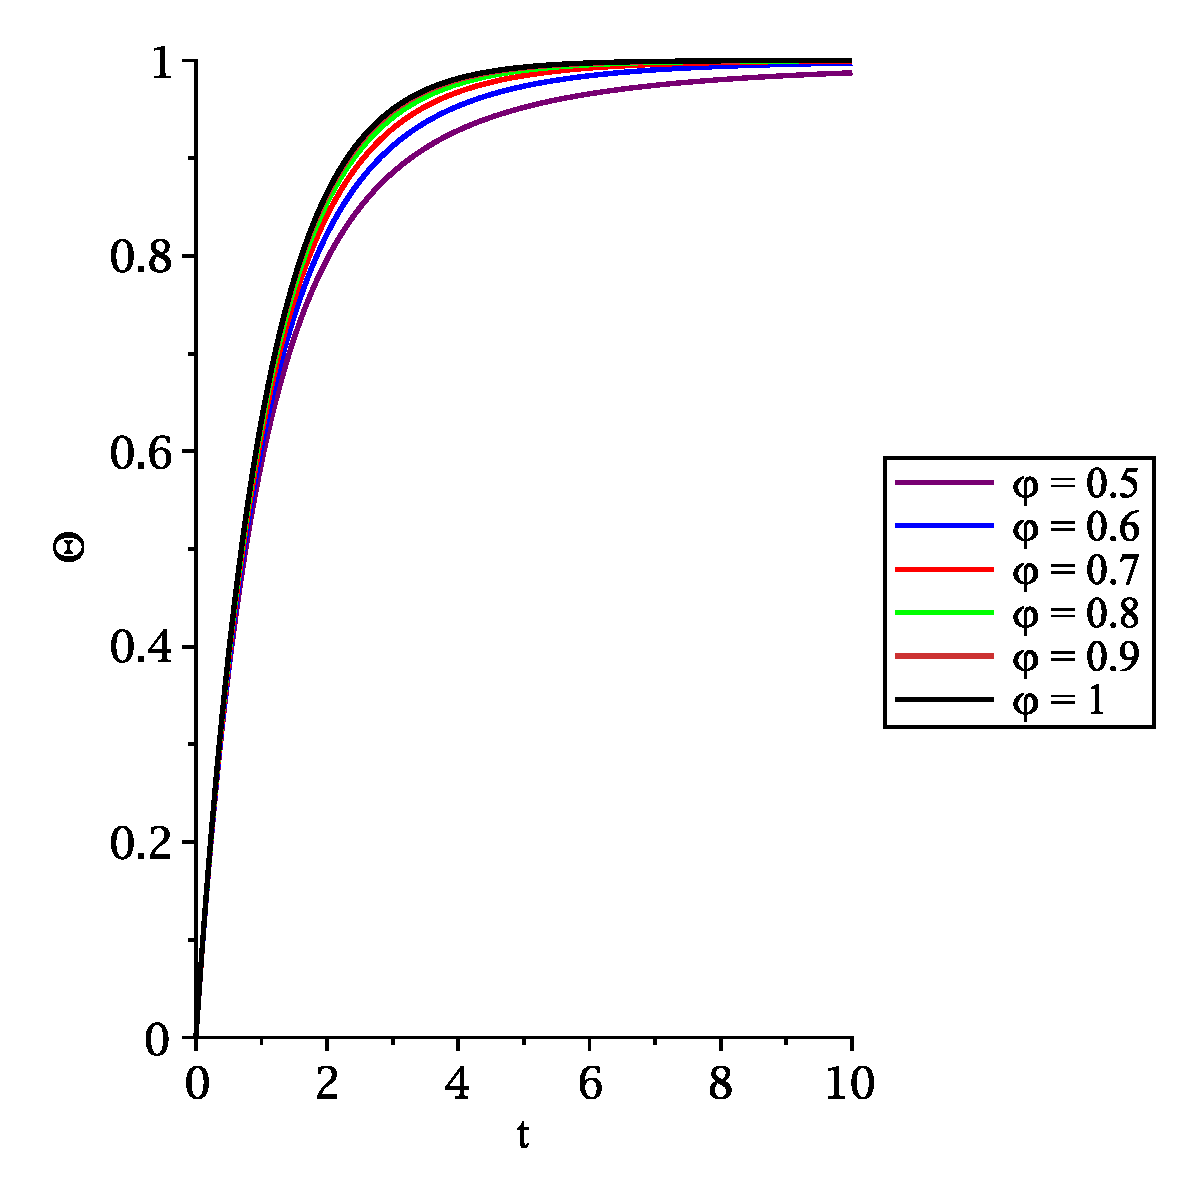
\includegraphics[scale = 0.35]{coverage_phi_02.eps}
	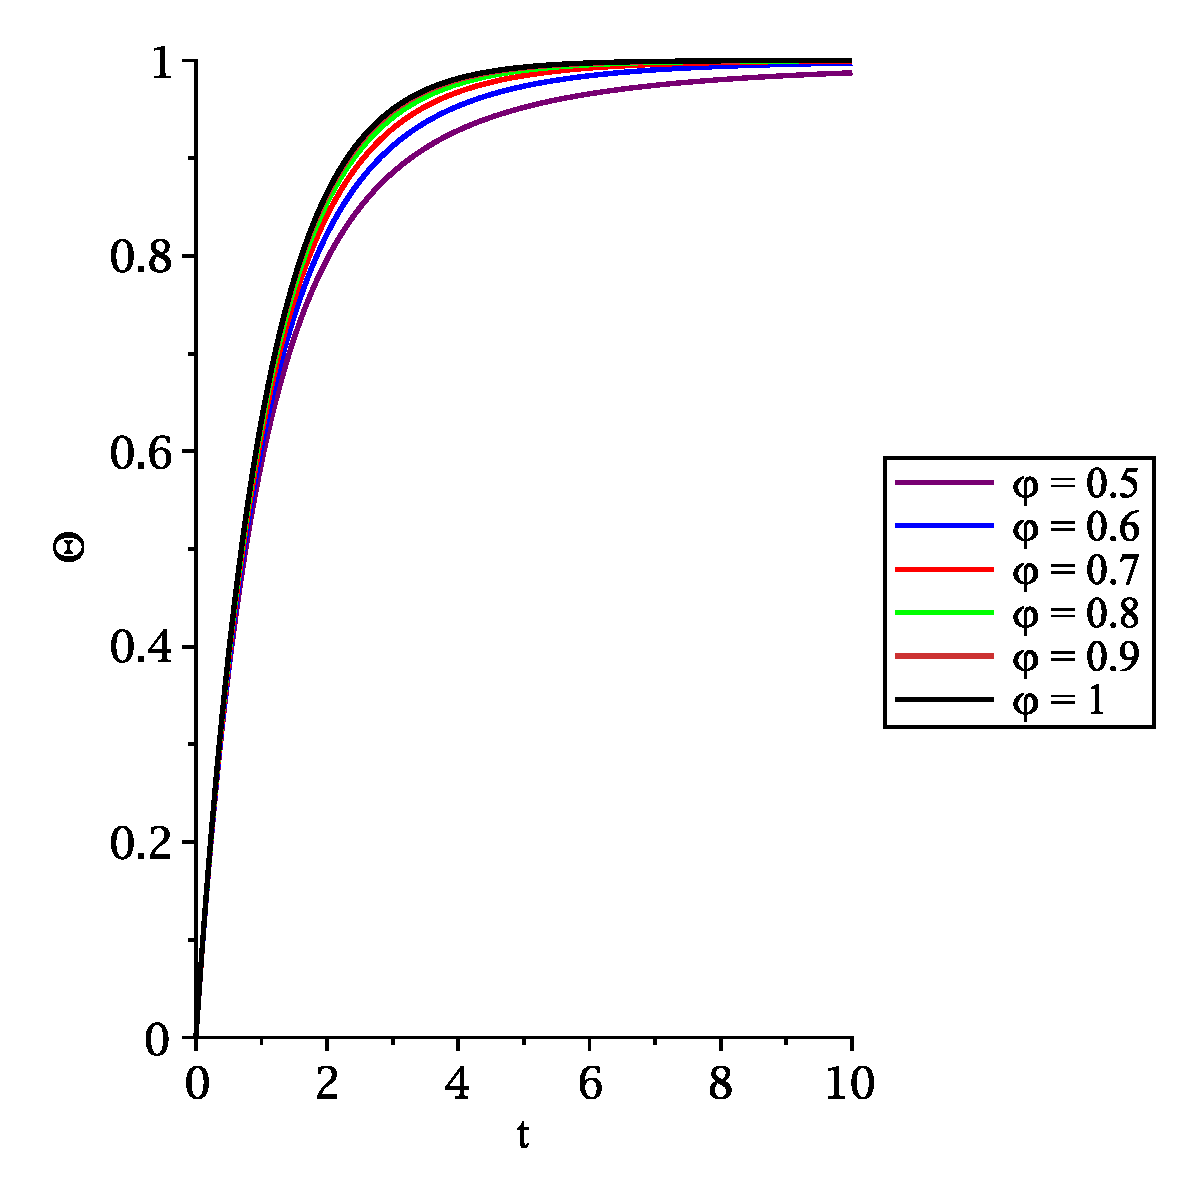
\includegraphics[width=\textwidth]{coverage_phi_02.eps}
	\caption{The coverage by cars}
	\label{fig:cp2}
\end{figure}\medskip

\newpage

We now consider the car coverage for $\phi = 1$. We first consider 
$F_{\phi}(t)$ when $\phi = 1$: \bigskip

\begin{eqnarray*}
	F_{\phi = 1}(t) & = & \exp \left( -2 \int_{0}^{t} \frac{(1 - e^{0})}{\tau} d\tau \right) \\\\
					& = & \exp \left( -2 \int_{0}^{t} \frac{(1 - 1)}{\tau} d\tau \right) \\\\
					& = & \exp \left( -2 \int_{0}^{t} \frac{0}{\tau} d\tau \right) \\\\
					& = & \exp \left( 0 \right) \\\\
					& = & 1
\end{eqnarray*}\medskip

making use of this we find: \bigskip

\begin{eqnarray*}
						\Theta_{\phi = 1}(t) & = & 1 - F_{\phi = 1}(t) e^{(1 - 2)t} \\\\
											 & = & 1 - e^{-t} \\\\
	\lim_{t \to \infty} \Theta_{\phi = 1}(t) & = & 1 - \lim_{t \to \infty} e^{-t} \\\\
											 & = & 1
\end{eqnarray*}\medskip

We now consider the car coverage for $\frac{1}{2} < \phi < 1$: \bigskip

\begin{eqnarray*}
	\lim_{t \to \infty} \Theta_{\phi}(t) & = & 1 - \lim_{t \to \infty} F_{\phi}(t) e^{(1 - 2 \phi)t} \\\\
										 & = & 1 - \lim_{t \to \infty} F_{\phi}(t) \cdot \lim_{t \to \infty} e^{-(2 \phi - 1)t} \\\\
										 & = & 1 - \lim_{t \to \infty} F_{\phi}(t) \cdot 0 \\\\
										 & = & 1 
\end{eqnarray*}\medskip

We now consider the car coverage for $\phi = \frac{1}{2}$. We first consider 
$F_{\phi}(t)$ when $\phi = \frac{1}{2}$: \bigskip

\begin{eqnarray*}
					 F_{\phi = 1/2}(t) & = & \exp \left( -2 \int_{0}^{t} \frac{(1 - e^{-\tau/2})}{\tau} d\tau \right) \\\\
									   & = & \exp \left( -2 \int_{0}^{t} \frac{1}{\tau} d\tau + 2 \int_{0}^{t} \frac{e^{-\tau/2}}{\tau} d\tau \right) \\\\
									   & = & \exp \left( -2 \int_{0}^{t} \frac{1}{\tau} d\tau\right) \cdot \exp \left( 2 \int_{0}^{t} \frac{e^{-\tau/2}}{\tau} d\tau \right) \\\\
									   & = & \exp \left( -2 \left. \ln(\tau) \right|_{\tau = 0}^{t} \right) \cdot \exp \left( 2 \int_{0}^{t} \frac{e^{-\tau/2}}{\tau} d\tau \right) \\\\
									   & = & \exp \left( - \left. \ln(\tau^2) \right|_{\tau = 0}^{t} \right) \cdot \exp \left( 2 \int_{0}^{t} \frac{e^{-\tau/2}}{\tau} d\tau \right) \\\\
									   & = & \exp \left( \ln\left( \frac{0}{t^2} \right) \right) \cdot \exp \left( 2 \int_{0}^{t} \frac{e^{-\tau/2}}{\tau} d\tau \right) \\\\
									   & = & \frac{0}{t^2} \cdot \exp \left( 2 \int_{0}^{t} \frac{e^{-\tau/2}}{\tau} d\tau \right) \\\\
	\therefore \quad F_{\phi = 1/2}(t) & = & 0
\end{eqnarray*}\medskip

and so we have: \bigskip

%\[
%	0 \leq F_{\phi = 1/2}(t) \leq 0 
%\]\medskip
%
%as $t \to \infty$, which implies: \bigskip
%
%\[
%	\lim_{t \to \infty} F_{\phi = 1/2}(t) = 0
%\]\medskip

\begin{eqnarray*}
	\Theta_{\phi = 1/2}(t) & = & 1 - F_{\phi = 1/2}(t) \\\\
%						   & = & 1 - F_{\phi = 1/2}(t) e^{0} \\\\
						   & = & 1 - 0 \\\\
						   & = & 1 
\end{eqnarray*}\medskip

hence if $\phi$ is at least $\frac{1}{2}$, then full coverage is achieved. In figure \ref{fig:cp3} 
we see the behaviour of the coverage for cars for values of $\phi$ between $0$ and $1$. \bigskip

\begin{figure}[h!]
	\centering
	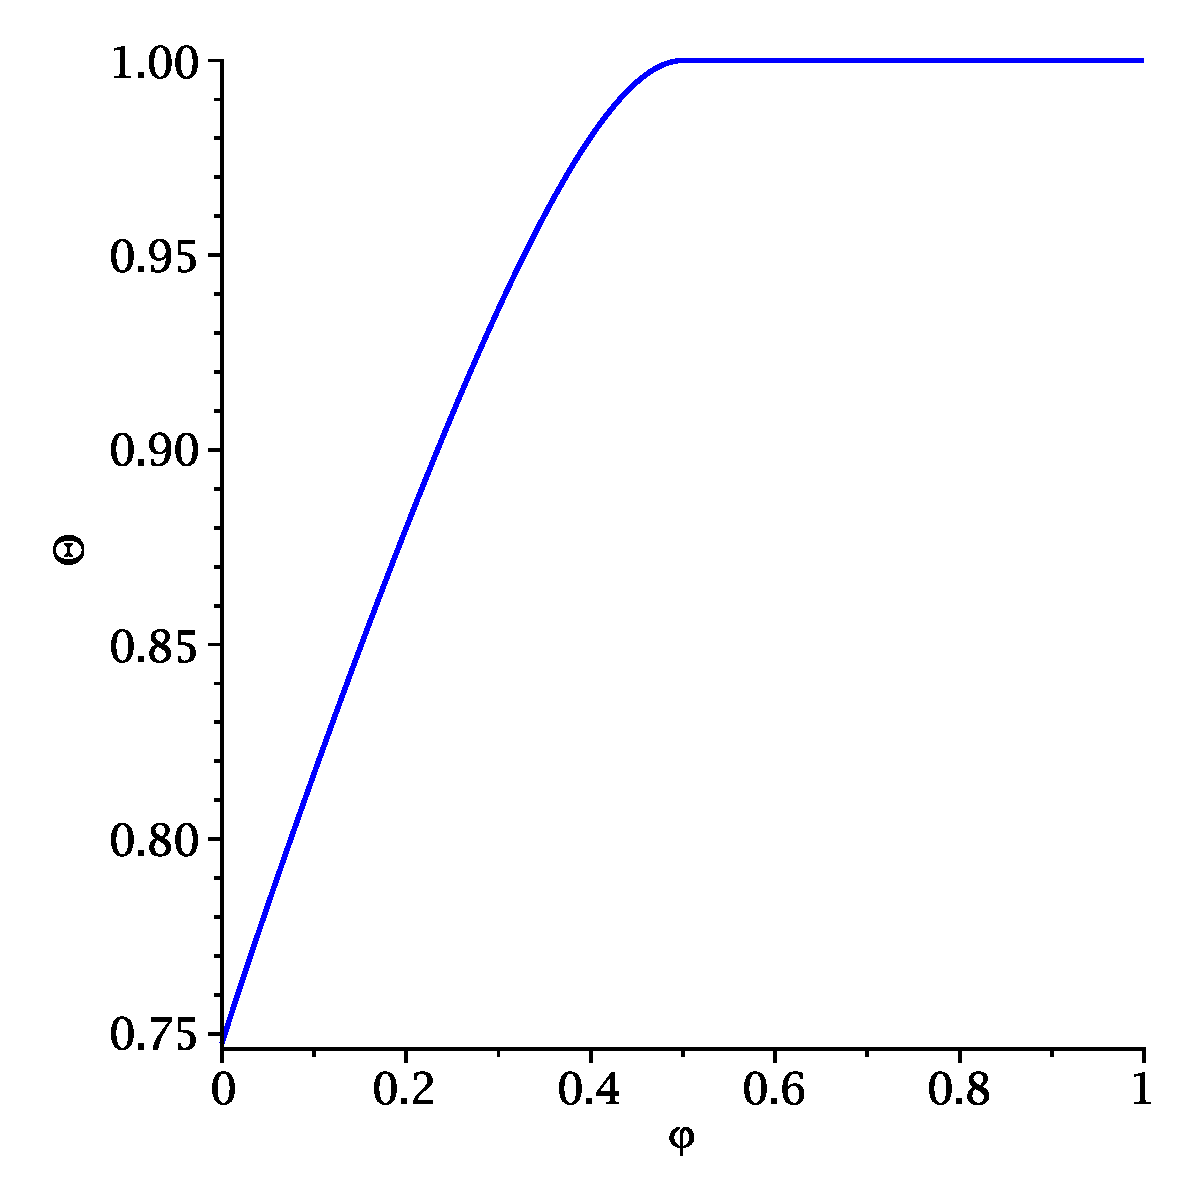
\includegraphics[scale = 0.35]{coverage_phi_03.eps}
%	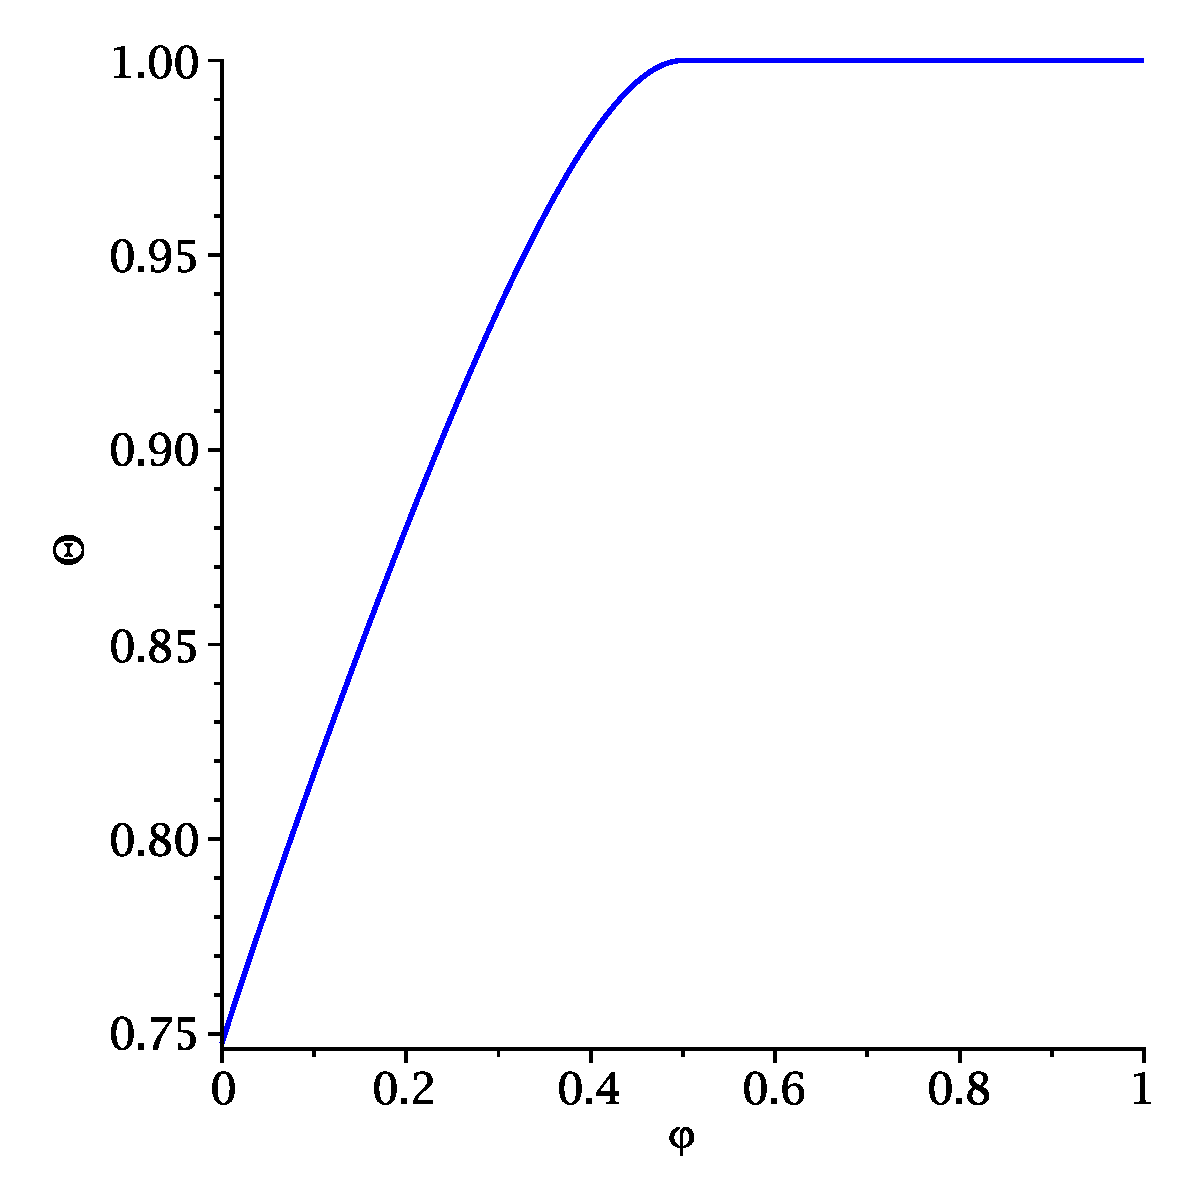
\includegraphics[width=\textwidth]{coverage_phi_03.eps}
	\caption{The coverage function as $t \to \infty$}
	\label{fig:cp3}
\end{figure}\medskip












\section{The reversible parking problem}

We now look at the reversible parking problem, where cars can both park and 
leave (see \cite{krapivsky1994collective}). In this version of the problem we 
assume that cars park at a rate of $k_{+}$ and leave at a rate of $k_{-}$. Thus 
far we have only considered the irreversible problem, which stops once the 
jamming limit has been reached. With the reversible problem we reach an 
equilibrium state when a balance is reached between the arrival rate $k_{+}$ 
and the leaving rate $k_{-}$. We define our rate equations for this case as 
follows, beginning with the $x < 1$ case: \bigskip

\[
	\frac{\partial P(x, t)}{\partial t} = -2 k_{-} P(x, t) + 2 k_{+} \int_{x + 1}^{\infty} P(y, t) dy  
\]\medskip

in which we have an adsorption ($+$) and a desorption ($-$) term. The adsorption 
term describes when a car parks within an interval of size $y > x + 1$, leaving a 
gap of length $x$, and this it can do in two different ways. The desorption term 
describes how a gap can be destroyed when any one of it's two neighbouring cars 
leaves. \bigskip

For the $x \geq 1$ case: \bigskip

\begin{eqnarray*}
	\frac{\partial P(x, t)}{\partial t} & = & -2 k_{-} P(x, t) + 2 k_{+} \int_{x + 1}^{\infty} P(y, t) dy \\\\
										&   &  -k_{+} (x - 1) P(x, t) + \frac{k_{-}}{\theta(t)} \int_{0}^{x - 1} P(y, t) P(x - 1 - y, t) dy 
\end{eqnarray*}\medskip

we have an additional two terms. The first describes how gaps of length greater 
than a car size are destroyed by arriving cars, with a rate $k_{+} (x - 1)$. The 
final term describes how two gaps separated by a car can form a larger gap when 
that car leaves. This term can be defined in terms of a gap-gap density function 
$P(y, z, t)$ which defines the density of neighbouring gaps of size $y$ and $z$ 
separated by a car. It can be defined as follows: \bigskip

\[
	P(y, z, t) = \frac{P(y, t) P(z, t)}{\theta(t)}
\]\medskip

In defining the gap-gap density function, we assume independence of the gap density 
functions, so that the distribution of two gaps separated by a single car is 
proportional to the product of the individual gap distributions. The coverage term 
in the denominator provides normalization. So the gap-gap density term above deals 
with the case where two neighbouring gaps, of size $y$ and $x - 1 - y$, separated 
by a single car, form a gap of size $x$ if the car separating the gaps leaves. \bigskip

From the above, it is clear that our condition for equilibrium is: \bigskip

\[
	\frac{\partial P(x, t)}{\partial t} = 0
\]\medskip

using the above rate equation we get: \bigskip

\begin{eqnarray*}
	-2 k_{-} P(x) + 2 k_{+} \int_{x + 1}^{\infty} P(y) dy & = & 0 \\\\
					2 k_{+} \int_{x + 1}^{\infty} P(y) dy & = & 2 k_{-} P(x) \\\\
							\int_{x + 1}^{\infty} P(y) dy & = & \frac{k_{-}}{k_{+}} P(x)
\end{eqnarray*}\medskip

using the substitution $P(x) = \beta e^{-\alpha x}$ we get: \bigskip

\begin{eqnarray*}
								  \int_{x + 1}^{\infty} \beta e^{-\alpha y} dy & = & \frac{k_{-}}{k_{+}} \beta e^{-\alpha x} \\\\
								  \beta \int_{x + 1}^{\infty} e^{-\alpha y} dy & = & \frac{k_{-}}{k_{+}} \beta e^{-\alpha x} \\\\
	\beta \left. \frac{ e^{-\alpha y} }{- \alpha} \right|_{y = x + 1}^{\infty} & = & \frac{k_{-}}{k_{+}} \beta e^{-\alpha x} \\\\
							  \frac{ e^{-\alpha} }{\alpha} \beta e^{-\alpha x} & = & \frac{k_{-}}{k_{+}} \beta e^{-\alpha x} \\\\
												  \frac{ e^{-\alpha} }{\alpha} & = & \frac{k_{-}}{k_{+}} \\\\
															 \alpha e^{\alpha} & = & \frac{k_{+}}{k_{-}} \\\\
\end{eqnarray*}\medskip

returning to our total coverage equation, and making the same substitution: \bigskip

\begin{eqnarray*}
														\int_{0}^{\infty} (x + 1) P(x) dx & = & 1 \\\\
								  \int_{0}^{\infty} x P(x) dx + \int_{0}^{\infty} P(x) dx & = & 1 \\\\
	\int_{0}^{\infty} x \beta e^{-\alpha x} dx + \int_{0}^{\infty} \beta e^{-\alpha x} dx & = & 1 \\\\
	\beta \int_{0}^{\infty} x e^{-\alpha x} dx + \beta \int_{0}^{\infty} e^{-\alpha x} dx & = & 1 \\\\
								\beta \left(\frac{1}{\alpha^2} + \frac{1}{\alpha} \right) & = & 1 \\\\
																	   \beta (1 + \alpha) & = & \alpha^2 \\\\
																					\beta & = & \frac{\alpha^2}{1 + \alpha} 
\end{eqnarray*}\medskip

which gives us for our equilibrium gap density function: \bigskip

\[
	P_{eq}(x) = \frac{\alpha^2}{1 + \alpha} e^{-\alpha x}
\]\medskip

We look next at the equilibrium coverage $\theta_{eq}$: \bigskip

\begin{eqnarray*}
	\theta_{eq} & = & \int_{0}^{\infty} P_{eq}(x) dx \\\\
				& = & \int_{0}^{\infty} \frac{\alpha^2}{1 + \alpha} e^{-\alpha x} dx \\\\
				& = & \frac{\alpha^2}{1 + \alpha} \int_{0}^{\infty} e^{-\alpha x} dx \\\\
				& = & \frac{\alpha^2}{1 + \alpha} \cdot \frac{1}{\alpha} \\\\
				& = & \frac{\alpha}{1 + \alpha} 
\end{eqnarray*}\medskip

And next we look at the function $\alpha \to \alpha e^{\alpha}$ on $(0, \infty)$: \bigskip

\begin{eqnarray*}
			 f(\alpha) & = & \alpha e^{\alpha} \\\\
	f^{\prime}(\alpha) & = & \alpha e^{\alpha} + e^{\alpha} \\\\
					   & = & (\alpha + 1) e^{\alpha} \\\\
					   & > & 0
\end{eqnarray*}\medskip

hence $f(\alpha)$ is strictly increasing on $(0, \infty)$. Therefore, if we were to 
graph the functions $y = f(\alpha)$ and $y = \frac{k_{+}}{k_{-}}$, they would meet 
in one and only one place, and hence there is a unique solution for 
$\alpha e^{\alpha} = \frac{k_{+}}{k_{-}}$. And also, as 
$\alpha e^{\alpha} = \frac{k_{+}}{k_{-}}$, if $\frac{k_{+}}{k_{-}} \to \infty$ 
then $\alpha e^{\alpha} \to \infty$ which implies $\alpha \to \infty$. In order to 
plot the equilibrium coverage as a function of $\frac{k_{+}}{k_{-}}$, we must first 
perform some manipulation: \bigskip

\begin{eqnarray*}
		 \alpha e^{\alpha} & = & \frac{k_{+}}{k_{-}} \\\\
	\ln(\alpha e^{\alpha}) & = & \ln \left( \frac{k_{+}}{k_{-}} \right) \\\\
	  \ln(\alpha) + \alpha & = & \ln \left( \frac{k_{+}}{k_{-}} \right) 
\end{eqnarray*}\medskip

Clearly, $\alpha$ dominates the left hand side as $\alpha \to \infty$, 
and hence: \bigskip

\[
	\alpha \approx \ln \left( \frac{k_{+}}{k_{-}} \right)
\]\medskip

putting this approximation for $\alpha$ into our expression for 
$\theta_{eq}$: \bigskip 

\begin{eqnarray*}
	\theta_{eq} & =       & \frac{\alpha}{1 + \alpha} \\\\
				& \approx & \frac{\alpha - 1}{\alpha} \quad \text{as } \alpha \to \infty \\\\
				& \approx & \frac{\ln(k_{+}/k_{-}) - 1}{\ln(k_{+}/k_{-})} \\\\
				& \approx & 1 - \frac{1}{\ln(k_{+}/k_{-})} 
\end{eqnarray*}\medskip

So we now have an approximation for the equilibrium coverage function as a 
function of $\frac{k_{+}}{k_{-}}$. In figure \ref{fig:ecf1} we see the behaviour 
of the equilibrium coverage function. We can see that $\theta_{eq}$ crosses $C_R$ 
(the red dashed line) as $\frac{k_{+}}{k_{-}}$ reaches approximately 50. \bigskip

\begin{figure}[h!]
	\centering
	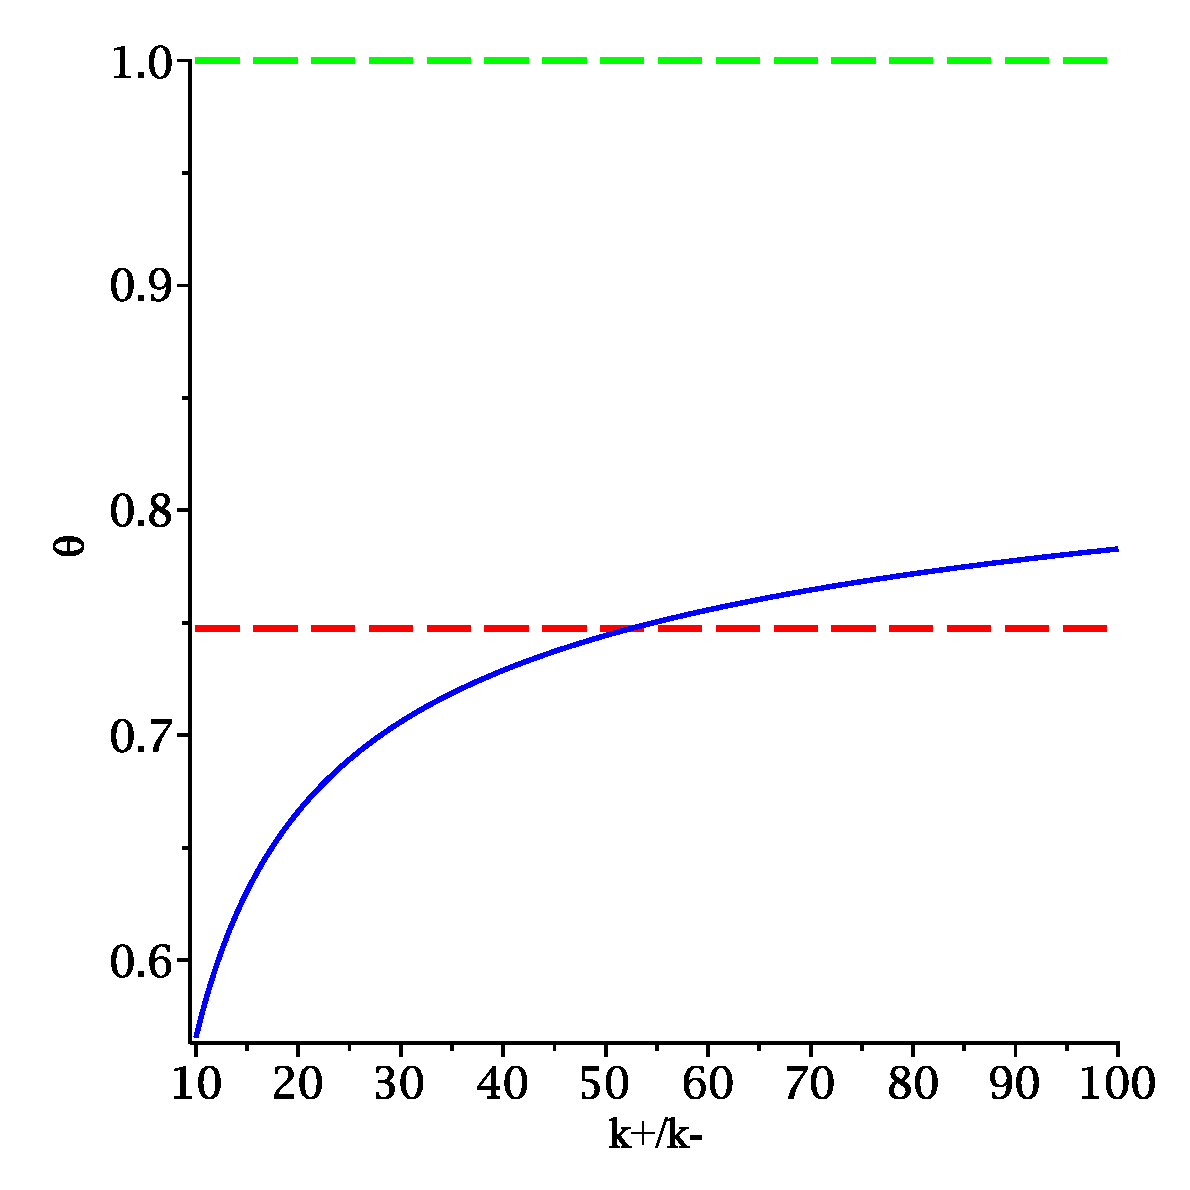
\includegraphics[scale = 0.35]{reversible_coverage_01.eps}
	%	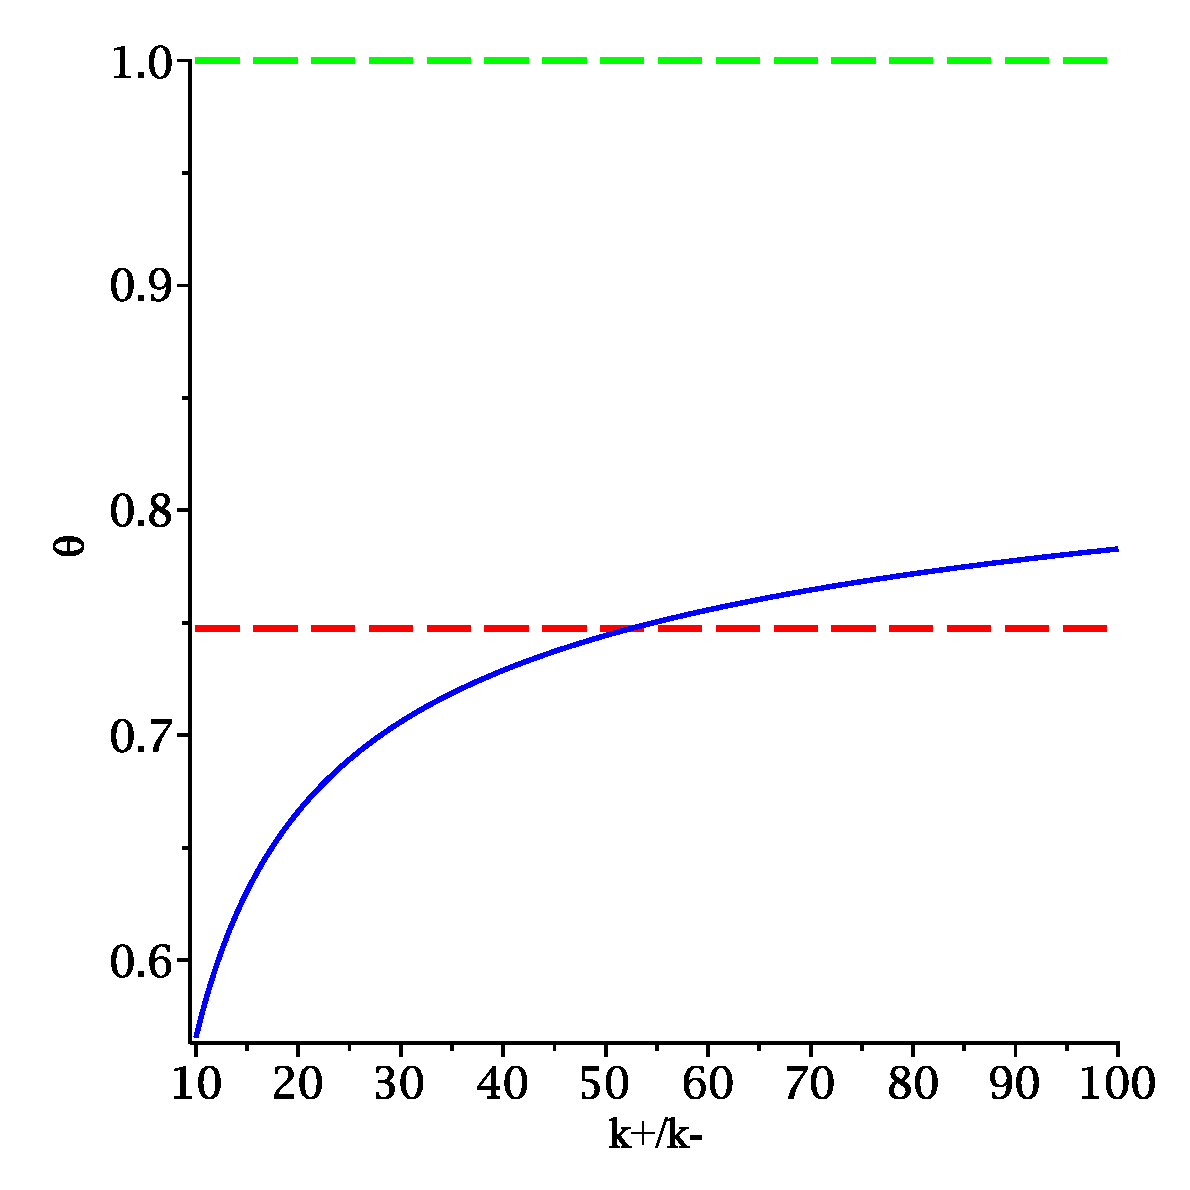
\includegraphics[width=\textwidth]{reversible_coverage_01.eps}
	\caption{The equilibrium coverage function}
	\label{fig:ecf1}
\end{figure}\medskip

In figure \ref{fig:ecf2} we see the behaviour of the equilibrium coverage 
function for a greater range of values of $\frac{k_{+}}{k_{-}}$. We can 
see that $\theta_{eq}$ continues to increase, albeit very slowly due to the 
logarithmic growth of the term involving $\frac{k_{+}}{k_{-}}$, towards $1$ 
(the green dashed line). \bigskip

\begin{figure}[h!]
	\centering
	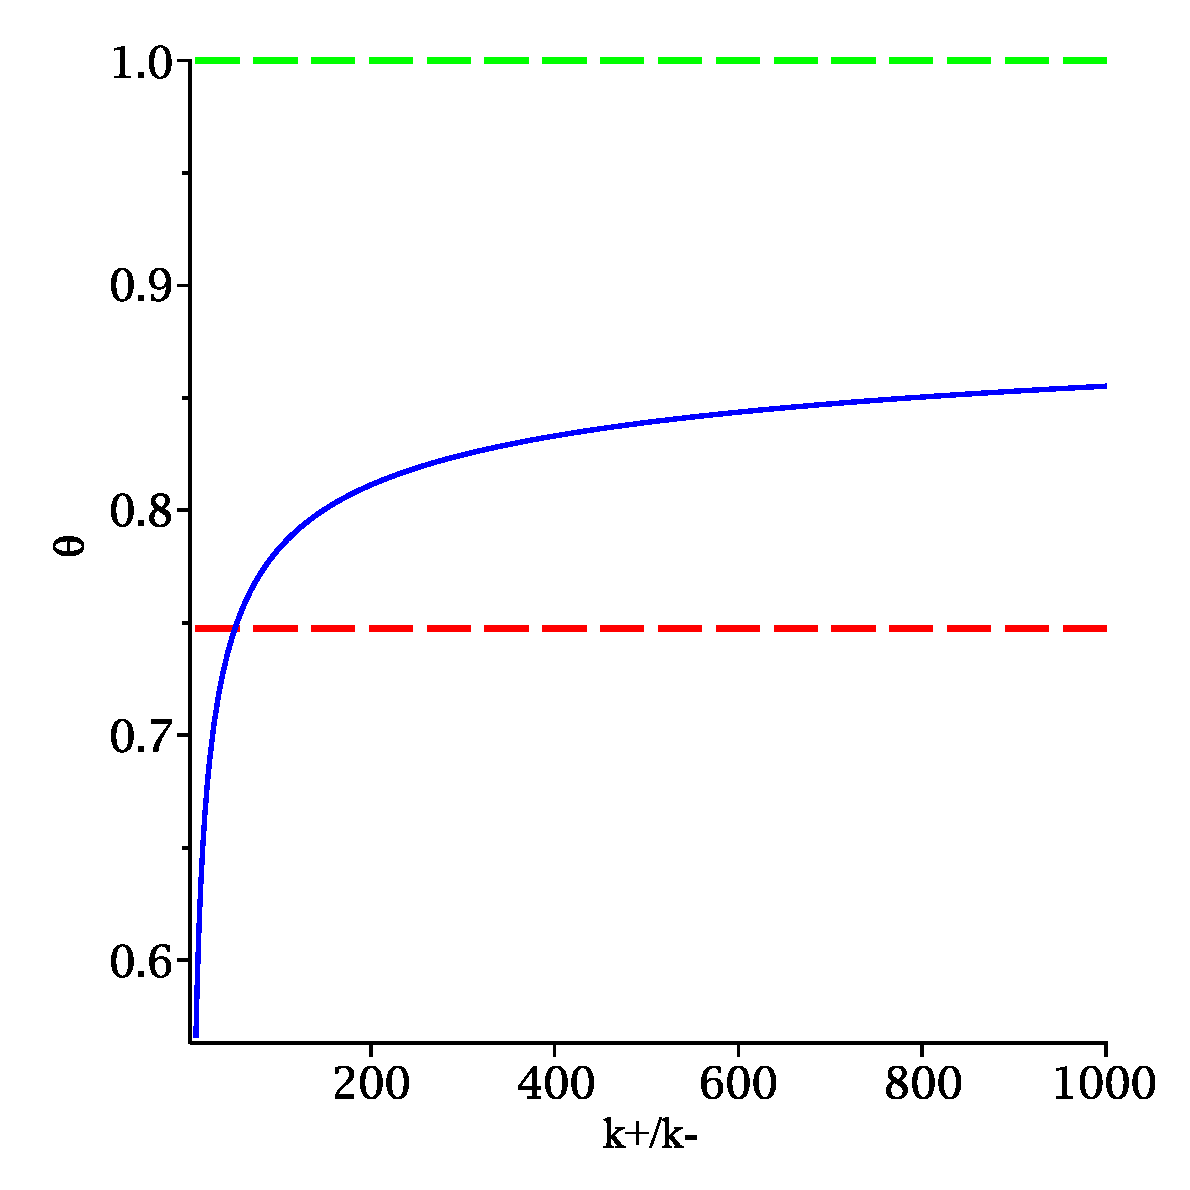
\includegraphics[scale = 0.35]{reversible_coverage_02.eps}
	%	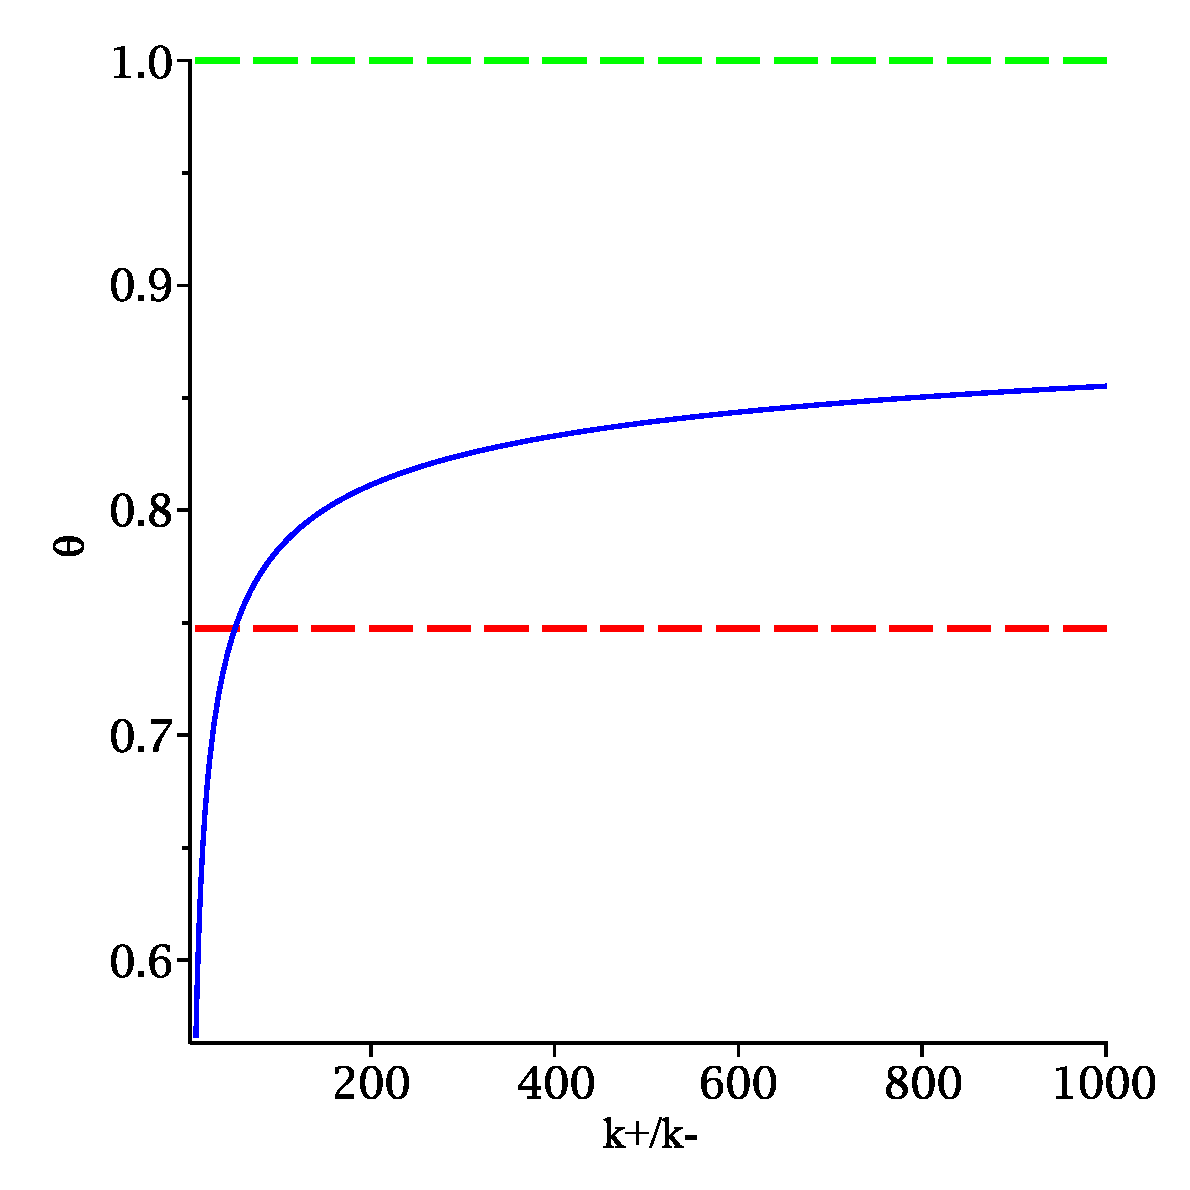
\includegraphics[width=\textwidth]{reversible_coverage_02.eps}
	\caption{The equilibrium coverage function}
	\label{fig:ecf2}
\end{figure}\medskip

It is easy to see from our approximation for the equilibrium coverage 
function that, as $\frac{k_{+}}{k_{-}} \to \infty$, 
$\ln\left(\frac{k_{+}}{k_{-}}\right) \to \infty$, and hence: \bigskip

\[
	\theta_{eq} \to 1 \quad \text{as } \frac{k_{+}}{k_{-}} \to \infty
\]\medskip

Where $k_{-} \to 0$, we have $\frac{k_{+}}{k_{-}} \to \infty$, and 
$\theta_{eq} \to 1$. So as $k_{-}$ gets closer to $0$, for example 
in the case where we can control desorption, the process tends towards 
full coverage. But in the case where $k_{-} = 0$, our problem collapses 
into the standard parking problem, and coverage falls back to $C_R$.











\section{Remarks}

As with the kinetic approach, we have successfully modelled the process with 
respect to it's time evolution, and with some generalizations. \bigskip

These solutions are even more satisfying than the kinetic approach because 
the assumptions of each extend the assumptions of the kinetic approach: \bigskip

\begin{itemize}
	\item \textbf{Kinetic Approach:} time evolution of parking cars
	\item \textbf{Overlap Approach:} time evolution of parking exclusion zones
	\item \textbf{Reversible Approach:} time evolution of cars that park and 
	leave at different rates
\end{itemize}\medskip

This can be seen in the construction of each of their rate equations, 
where the rate equations for each generalization builds on the rate 
equations of the kinetic approach by adding extra terms reflecting 
the extra sophistication. \bigskip













\chapter{Simulations}











\section{Introduction}

Many of the solutions we have covered in this paper require 
numerical techniques for evaluation. We present a different 
approach that serves as both a means of evaluating results, 
and as a way of confirming theories. \bigskip

%For example: \bigskip
%
%\[
%	C_R = \int_{0}^{\infty} \exp \left( -2 \int_{0}^{t} \frac{1 - e^{-u}}{u} du \right) dt
%\]\medskip
%
%which can only be evaluated numerically. 

The Monte Carlo approach is a computational technique that 
is best applied to problems that have a probabilistic 
element. The technique can be summarized as follows: \bigskip

\begin{itemize}
	\item define the range of values to be drawn from
	\item draw values from this range using a distribution
	\item perform a computation on the results 
	\item record the results of the computation
	\item repeat as appropriate
\end{itemize}\medskip

So in the case of the parking problem, the steps would 
be as follows: \bigskip

\begin{itemize}
	\item define the length $L$ on which cars can be parked
	\item draw values from the interval $(0, L)$ using a 
	distribution to simulate the spots taken by cars parking 
	on the length $L$
	\item once no more parking spots remain calculate the 
	coverage, in this case the ratio of cars to the length $L$
	\item record the results of this computation
	\item repeat for as many iterations as required and 
	present statistics of the results of the simulation
\end{itemize}\medskip

The results of the simulation serve as both an estimation 
of a value, but can also be used to confirm that a theory 
is valid where experimental verification might be 
difficult or impractical. \bigskip

We will initially illustrate the usefulness of this approach  
by looking at a simple variation on the parking problem, the 
discrete parking problem (see \cite{krapivsky2010kinetic}), 
where we have an exact result that is easy to evaluate, and 
demonstrate that the technique produces results that are 
consistent with the theory. \bigskip

\newpage






\section{The Discrete Parking Problem}

In the discrete parking problem we have a length $L$ 
made up of discrete sites, and we attempt to park cars 
that occupy two adjacent sites. If a car tries to park 
at two adjacent empty sites, the process is successful, 
otherwise unsuccessful. The process continues until 
there are no more free adjacent empty sites that can 
accommodate cars. \bigskip

The coverage for the discrete parking 
problem is $\theta_{d}(t)$, and the jamming coverage is: \bigskip

\[
	\lim_{t \to \infty} \theta_{d}(t) = 1 - e^{-2}
\]\medskip

which is calculated to be $0.864664$ to six decimal 
places. Below we see the output of a simulation for this problem 
where the number of iterations is set to $10000$ and the 
length $L$ is set to $100000$: \bigskip

%\begin{mdframed}
	\begin{lstlisting}[numbers=none]
    Parking Problem - Discrete Version: results

                                     L:   100000
                            iterations:    10000

                          distribution:
                                  mean: 0.864673
                    standard deviation: 0.000848

	\end{lstlisting} \bigskip
%\end{mdframed} \bigskip

In figure \ref{fig:ps1} we see a plot of the distribution 
of results from our simulation. It has the familiar bell 
curve shape which would imply the simulation produces 
results that are normal, or nearly normal, which in turn 
tells us, for example, that $95\%$ of the results are 
within $2$ standard deviations of the mean. This in itself 
should give us confidence in the technique. \bigskip

\begin{figure}[h!]
	\centering
	\includegraphics[scale = 0.65]{parking_simulation_01.eps}
%	\includegraphics[width=\textwidth]{parking_simulation_01.eps}
	\caption{Histogram of the parking problem simulation - discrete case}
	\label{fig:ps1}
\end{figure}\medskip

So with not much effort we seem to have arrived at an 
alternative approach to numerical techniques for 
evaluation of sometimes complicated results. We see 
consistency between the result calculated above, and 
from our simulation, which would seem to validate the 
mathematics. \bigskip

%\newpage








\section{The Parking Problem}

Next we will simulate the parking problem. We construct 
the simulation similarly to the discrete case, except 
in this case we do not park in discrete adjacent places, 
so our implementation is actually simpler. The jamming 
coverage for the parking problem is: \bigskip

\[
	C_R = \int_{0}^{\infty} \exp \left( -2 \int_{0}^{t} \frac{1 - e^{-u}}{u} du \right) dt
\]\medskip

which can only be evaluated numerically, and is 
calculated to be $0.747598$ to six decimal places. We 
see below the output of a simulation for this problem 
with the number of iterations set to $10000$ and $L$ 
set to $100000$: \bigskip

%\begin{mdframed}
	\begin{lstlisting}[numbers=none]
                    Parking Problem: results

                                  L:   100000
                         iterations:    10000

                       distribution:
                               mean: 0.747602
                 standard deviation: 0.000617

	\end{lstlisting} \bigskip
%\end{mdframed} \bigskip

In figure \ref{fig:ps2} we see a plot of the distribution 
of results from our simulation. Once again, we see the 
familiar bell curve shape which would again imply the 
simulation produces results that are normal, or nearly 
normal. \bigskip

\begin{figure}[h!]
	\centering
	\includegraphics[scale = 0.65]{parking_simulation_02.eps}
%	\includegraphics[width=\textwidth]{parking_simulation_02.eps}
	\caption{Histogram of the parking problem simulation}
	\label{fig:ps2}
\end{figure}\medskip

Once again we see clear consistency between the numerically 
evaluated result, and the result of the simulation. So again 
we have provided a pretty successful means of evaluating our 
constant other than the standard numerical approach. \bigskip

%\newpage







\section{Parking with overlap}

Next we will simulate parking with overlap. We construct 
the simulation similarly to the earlier cases, except 
in this case we park by exclusion zone. The coverage by 
cars for parking with overlap is: \bigskip

\begin{eqnarray*}
	\Theta_{\phi}(t) = 
	\begin{dcases}
		(1 - 2 \phi) \int_{0}^{t} F_{\phi}(\tau) d \tau  + \int_{0}^{t} F_{\phi}(\tau) \frac{2}{\tau} (1 - e^{-\phi \tau}) d \tau			& \text{for } \phi < \frac{1}{2} \\\\
		1 - F_{\phi}(t) e^{(1 - 2 \phi)t}																									& \text{for } \phi \geq \frac{1}{2} 
	\end{dcases}
\end{eqnarray*}\medskip

The jamming coverage for a selection of values for $\phi$ 
as $t \to \infty$ is shown below in table \ref{table:2}: \bigskip

\begin{table}[h!]
	\centering
	\begin{tabular}{|l | l|} 
		\hline
		$\phi$ & $\lim_{t \to \infty} \Theta_{\phi}(t)$ \\ [1ex] 
		\hline
		0.1 & 0.816909 \\ 
		0.2 & 0.880028 \\ 
		0.3 & 0.936238 \\ 
		0.4 & 0.980342 \\ 
		0.5 & 1 \\ 
		\hline
	\end{tabular}
	\caption{$\lim_{t \to \infty} \Theta_{\phi}(t)$}
	\label{table:2}
\end{table}\medskip

As we see, the coverage gets closer to full coverage (i.e. $1$) 
as $\phi \to 0.5$. \bigskip

\newpage

We see below the output of a simulation for this problem with 
the number of iterations set to $10000$, $L$ set to $100000$, 
and with $\phi$ set to $0.1$: \bigskip

%\begin{mdframed}
	\begin{lstlisting}[numbers=none]
    Parking Problem - Overlap Version: results

                                    L:   100000
                              overlap:      0.1
                           iterations:    10000

                         distribution:
                                 mean: 0.816894
                   standard deviation: 0.000584

	\end{lstlisting} \bigskip
%\end{mdframed} \bigskip

In figure \ref{fig:ps3} we see a plot of the distribution 
of results from our simulation for $\phi = 0.1$: \bigskip

\begin{figure}[h!]
	\centering
	\includegraphics[scale = 0.65]{parking_simulation_03.eps}
	%	\includegraphics[width=\textwidth]{parking_simulation_03.eps}
	\caption{Histogram of the parking with overlap simulation - $\phi = 0.1$}
	\label{fig:ps3}
\end{figure}\medskip

\newpage

We see below the output of a simulation for this 
problem with the number of iterations set to $10000$, 
$L$ set to $100000$, and with $\phi$ set to $0.2$: \bigskip

%\begin{mdframed}
	\begin{lstlisting}[numbers=none]
    Parking Problem - Overlap Version: results
	
                                    L:   100000
                              overlap:      0.2
                           iterations:    10000
	
                         distribution:
                                 mean: 0.880027
                   standard deviation: 0.000477

	\end{lstlisting} \bigskip
%\end{mdframed} \bigskip

In figure \ref{fig:ps4} we see a plot of the distribution 
of results from our simulation for $\phi = 0.2$: \bigskip

\begin{figure}[h!]
	\centering
	\includegraphics[scale = 0.65]{parking_simulation_04.eps}
	%	\includegraphics[width=\textwidth]{parking_simulation_04.eps}
	\caption{Histogram of the parking with overlap simulation - $\phi = 0.2$}
	\label{fig:ps4}
\end{figure}\medskip

\newpage

We see below the output of a simulation for this 
problem with the number of iterations set to $10000$, 
$L$ set to $100000$, and with $\phi$ set to $0.3$: \bigskip

%\begin{mdframed}
	\begin{lstlisting}[numbers=none]
    Parking Problem - Overlap Version: results

                                    L:   100000
                              overlap:      0.3
                           iterations:    10000

                         distribution:
                                 mean: 0.936235
                   standard deviation: 0.000327

	\end{lstlisting} \bigskip
%\end{mdframed} \bigskip

In figure \ref{fig:ps5} we see a plot of the distribution 
of results from our simulation for $\phi = 0.3$: \bigskip

\begin{figure}[h!]
	\centering
	\includegraphics[scale = 0.65]{parking_simulation_05.eps}
	%	\includegraphics[width=\textwidth]{parking_simulation_05.eps}
	\caption{Histogram of the parking with overlap simulation - $\phi = 0.3$}
	\label{fig:ps5}
\end{figure}\medskip

\newpage

We see below the output of a simulation for this 
problem with the number of iterations set to $10000$, 
$L$ set to $100000$, and with $\phi$ set to $0.4$: \bigskip

%\begin{mdframed}
	\begin{lstlisting}[numbers=none]
    Parking Problem - Overlap Version: results

                                    L:   100000
                              overlap:      0.4
                           iterations:    10000

                         distribution:
                                 mean: 0.980344
                   standard deviation: 0.000144

	\end{lstlisting} \bigskip
%\end{mdframed} \bigskip

In figure \ref{fig:ps6} we see a plot of the distribution 
of results from our simulation for $\phi = 0.4$: \bigskip

\begin{figure}[h!]
	\centering
	\includegraphics[scale = 0.65]{parking_simulation_06.eps}
	%	\includegraphics[width=\textwidth]{parking_simulation_06.eps}
	\caption{Histogram of the parking with overlap simulation - $\phi = 0.4$}
	\label{fig:ps6}
\end{figure}\medskip

\newpage

We see below the output of a simulation for this 
problem with the number of iterations set to $10000$, 
$L$ set to $100000$, and with $\phi$ set to $0.5$: \bigskip

%\begin{mdframed}
	\begin{lstlisting}[numbers=none]
    Parking Problem - Overlap Version: results

                                    L:   100000
                              overlap:      0.5
                           iterations:    10000

                         distribution:
                                 mean: 1.000000
                   standard deviation: 0.000000

	\end{lstlisting} \bigskip
%\end{mdframed} \bigskip

In figure \ref{fig:ps7} we see a plot of the distribution 
of results from our simulation for $\phi = 0.5$: \bigskip

\begin{figure}[h!]
	\centering
	\includegraphics[scale = 0.65]{parking_simulation_07.eps}
%	\includegraphics[width=\textwidth]{parking_simulation_07.eps}
	\caption{Histogram of the parking with overlap simulation - $\phi = 0.5$}
	\label{fig:ps7}
\end{figure}\medskip

\newpage

So again we see strong consistency between the results 
of our simulations, and the corresponding calculated results. 
And the consistent results serve to verify our approach. \bigskip















\section{Remarks}

There are two approaches to implementing simulations: \bigskip

\begin{itemize}
	\item an iterative approach - ordinarily more faithful to the problem, 
	but can take a long time to complete
	\item a recursive approach - more suited to evaluating results, and 
	completes relatively quickly
\end{itemize}\medskip

In the context of our simulations, if we want to confirm that we have 
modelled the process correctly, we might choose an iterative implementation, 
in which case the outcome will be more accurate the more iterations we 
perform, and for larger values of $L$, but if the number of iterations is 
too great, and if $L$ is too large, then the simulation may take a very long 
time to complete. \bigskip

So there needs to be a trade-of made: \bigskip

\begin{itemize}
	\item if high accuracy of the outcome is required, then you should 
	use lots of iterations, and set $L$ to be as large as possible
	\item if confirmation of a theory is all that is required, then 
	fewer iterations will be necessary, and a shorter $L$ will suffice
	\item if the calculation of a value is required, then the recursive 
	approach should be used
\end{itemize}\medskip













\chapter{Conclusions}











\section{Remarks}

The kinetic approach is wholly satisfying, and leaves the way open to further research. 
This author was struck by the elegance of the derivations, and spent some time considering 
whether or not there was some underlying conservation law other than the obvious: \bigskip

\[
	\int_{0}^{\infty} x P(x, t) dx + \int_{0}^{\infty} P(x, t) dx = 1
\]\medskip

i.e that the normalized sum of the car lengths and gap lengths equals 1. And with respect to 
the generalizations of the kinetic framing of the problem, once again we see two beautifully 
elegant solutions. In particular, the reversible problem, and it's condition for equilibrium: \bigskip

\[
	\frac{\partial P(x, t)}{\partial t} = 0
\]\medskip

which would lead one to believe that there are hidden symmetries. \bigskip

We have demonstrated that the general approach of validating theory through simulations has 
been useful. When it comes to modelling a problem that does not lend itself easily to 
empirical verification, such as the parking problem, a simulation can tell you if your theory 
makes sense very quickly. \bigskip

Also, we have shown that simulations can help to provide statistical properties relating to 
the associated constants, which in turn can help establish whether a process is being 
inhibited by some unknown factor - for example, if an adsorption yield in some industrial 
process falls outside of $2$ standard deviations of the mean yield from a simulation based 
on the existing conditions, then some investigation might be warranted. \bigskip











\section{Future Research}

In this author's view there is scope for further research into the derivation of the 
time-independent limit, in the one-dimensional case, which does not take R\'enyi's 
approach. Also, the jamming limit $C_R$ feels like something universal, akin to $e$ 
or $\phi$, or even $\pi$. It feels like the surface was only scratched and a much more 
satisfying number-theoretic approach could be taken. This author would welcome such 
research. \bigskip

This author also believes that there may be more interesting results, and possibly 
hidden symmetries found, from studying this problem in the context of distributions 
- both in the specific probabilistic, and more general special function, sense. \bigskip

Higher dimensional problems, in two and three dimensions, would be a logical next 
research topic - investigating what (if any) relationship exists between two and 
three dimensional packing problems and $C_R$. \bigskip

Sadly, one generalization I did not have time to look at in much depth is 
\emph{Competitive RSA of a binary mixture}, where cars of two different lengths 
compete for parking spaces. This is a more complicated problem mathematically, and 
is actually more difficult to simulate, but might have more general, or practical, 
applications. This author feels this subject is certainly worthy of more attention. \bigskip














\appendix


\chapter{The Simulation Code}

All simulations were implemented in Python. Two implementations were provided 
for each simulation - a recursive and an iterative implementation. The driver 
code for each implementation was similar in each case, with the required 
differences located in one or more extra functions. I will provide listings 
of the main simulation driver code, and then the different functions that 
contain the unique implementations for the respective simulations. \bigskip

In listing \ref{lst:code1} we see the code that runs the simulations and 
aggregates the results of each simulation. \bigskip

%\begin{mdframed}
\begin{lstlisting}[language=python,caption=Parking Problem - simulation driver,label=lst:code1]
	def simulation(iterations, length):
		results = []
		
		print()
		print(' Parking Problem: running {} simulations'.format(iterations))
		print()
	
		for i in range(iterations):
			results.append(parking_problem(length))
	
		print('          L: {:8d}'.format(length))
		print(' iterations: {:8d}'.format(iterations))
		print()
		
		return results

\end{lstlisting} \bigskip
%\end{mdframed} \bigskip

In listing \ref{lst:code2} we see the recursive implementation of the code 
that parks the cars and calculates the required ratio for the standard case. \bigskip

%\begin{mdframed}
\begin{lstlisting}[language=python,caption=Parking Problem - Recursive - standard case,label=lst:code2]
	def parking_problem(length):
		spots = []
		
		def find_spots(start, end):
			spot = np.random.uniform(start, end)
			spots.append(spot)
			
			if start <= spot - 1.0:
				find_spots(start, spot - 1.0)
			
			if spot + 1.0 <= end:
				find_spots(spot + 1.0, end)
		
		find_spots(0, length)
		
		return len(spots) / float(length)

\end{lstlisting}  \bigskip
%\end{mdframed} \bigskip

In listing \ref{lst:code2.5} we see the iterative implementation of the code 
that parks the cars and calculates the required ratio for the standard case. 
We can see that there are extra functions to check if there are available parking 
spots on the line, to check if a spot can be occupied by a car, and to draw 
a parking spot uniformly from the line. The main function retrieves a parking 
spot, if a car fits in the spot it is parked, and iterates in this fashion 
until there are no more spots available for parking. A counter is maintained 
that prevents the iterative function from continuing indefinitely. \bigskip

%\begin{mdframed}
\begin{lstlisting}[language=python,caption=Parking Problem - Iterative - standard case,label=lst:code2.5]
	def spots_available(spots, length):
		if 0 <= spots[0] - 1.0:
			return True

		for i in range(len(spots) - 1):
			if spots[i] + 1.0 <= spots[i + 1] - 1.0:
				return True

		return spots[-1] + 1 <= length - 1.0

	def spot_found(spot, spots, length):
		if 0 <= spot <= spots[0] - 1.0:
			return True

		for i in range(len(spots) - 1):
			if spots[i] + 1.0 <= spot <= spots[i + 1] - 1.0:
				return True

		return spots[-1] + 1.0 <= spot <= length - 1.0

	def get_parking(length):
		return np.random.uniform(0, length)

	def parking_problem(length):
		spots = [get_parking(length)]
		count = 0

		while spots_available(spots, length):
			spot = get_parking(length)

			if spot_found(spot, spots, length):
				spots.append(spot)
				spots.sort()

			count += 1

			if count == 10000000:
				break

		return len(spots) / float(length)

\end{lstlisting}  \bigskip
%\end{mdframed} \bigskip

In listing \ref{lst:code3} we see the recursive implementation of the code 
that parks the cars and calculates the required ratio for the discrete case. \bigskip

%\begin{mdframed}
\begin{lstlisting}[language=python,caption=Parking Problem - Recursive - discrete case,label=lst:code3]
	def parking_problem(length):
		spots = []

		def find_spots(start, end):
			spot = np.random.randint(start, end)
			spots.append(spot)

			if start <= spot - 2:
				find_spots(start, spot - 1)

			if spot + 3 <= end:
				find_spots(spot + 2, end)

		find_spots(0, length)

		return (len(spots) * 2) / float(length)

\end{lstlisting}  \bigskip
%\end{mdframed} \bigskip

In listing \ref{lst:code3.5} we see the iterative implementation of the code 
that parks the cars and calculates the required ratio for the discrete case. 
Similar to the standard case, there are extra functions provided with the 
difference being that the car length is set to $2$, and an integer parking 
spot is drawn from the line. \bigskip

%\begin{mdframed}
\begin{lstlisting}[language=python,caption=Parking Problem - Iterative - discrete case,label=lst:code3.5]
	def spots_available(spots, length):
		if 0 <= spots[0] - 2:
			return True

		for i in range(len(spots) - 1):
			if spots[i] + 2 <= spots[i + 1] - 2:
				return True

		return spots[-1] + 2 <= length - 1

	def spot_found(spot, spots, length):
		if 0 <= spot <= spots[0] - 2:
			return True

		for i in range(len(spots) - 1):
			if spots[i] + 2 <= spot <= spots[i + 1] - 2:
				return True

		return spots[-1] + 2 <= spot <= length - 1

	def get_parking(length):
		return np.random.randint(0, length)

	def parking_problem(length):
		spots = [get_parking(length)]
		count = 0

		while spots_available(spots, length):
			spot = get_parking(length)

			if spot_found(spot, spots, length):
				spots.append(spot)
				spots.sort()

			count += 1

			if count == 10000000:
				break

		return (len(spots) * 2) / float(length)

\end{lstlisting}  \bigskip
%\end{mdframed} \bigskip

In listing \ref{lst:code4} we see the recursive implementation of the code 
that parks the cars and calculates the required ratio for the overlap case. 
For the overlap case we have added an extra function for calculating the total  
length of the gaps. This is necessary in the overlap case precisely because 
cars can overlap when they park, and hence the number of cars can not be used 
as a measure of the coverage. \bigskip

%\begin{mdframed}
\begin{lstlisting}[language=python,caption=Parking Problem - Recursive - overlap case,label=lst:code4]
	def parking_problem(length, overlap):
		exclusion = 1.0 - overlap
		spots     = []
		
		def find_spots(start, end):
			spot = np.random.uniform(start, end)
			spots.append(spot)
			
			if start <= spot - exclusion:
				find_spots(start, spot - exclusion)
			
			if spot + exclusion <= end:
				find_spots(spot + exclusion, end)
		
		find_spots(0, length)
		
		return (length - total_gaps(sorted(spots))) / float(length)
	
	def total_gaps(spots):
		total = 0
		
		for i in range(len(spots) - 1):
			value = spots[i + 1] - (spots[i] + 1)
			if value > 0:
				total += value 
		
		value = spots[-1] - (spots[-2] + 1)
		if value > 0:
			total += value 
		
		return total

\end{lstlisting}  \bigskip
%\end{mdframed} \bigskip

In listing \ref{lst:code4.5} we see the iterative implementation of the code 
that parks the cars and calculates the required ratio for the overlap case. \bigskip

%\begin{mdframed}
\begin{lstlisting}[language=python,caption=Parking Problem - Iterative - overlap case,label=lst:code4.5]
	def spots_available(spots, length, overlap):
		exclusion = 1.0 - overlap

		if 0 <= spots[0] - exclusion:
			return True

		for i in range(len(spots) - 1):
			if spots[i] + exclusion <= spots[i + 1] - exclusion:
				return True

		return spots[-1] + exclusion <= length - exclusion

	def spot_found(spot, spots, length, overlap):
		exclusion = 1.0 - overlap

		if 0 <= spot <= spots[0] - exclusion:
			return True

		for i in range(len(spots) - 1):
			if spots[i] + exclusion <= spot <= spots[i + 1] - exclusion:
				return True

		return spots[-1] + exclusion <= spot <= length - exclusion

	def get_parking(length):
		return np.random.uniform(0, length)

	def total_gaps(spots):
		total = 0

		for i in range(len(spots) - 1):
			value = spots[i + 1] - (spots[i] + 1)
			if value > 0:
				total += value 

		value = spots[-1] - (spots[-2] + 1)
		if value > 0:
			total += value 

		return total

	def parking_problem(length, overlap):
		spots = [get_parking(length)]
		count = 0

		while spots_available(spots, length, overlap):
			spot = get_parking(length)

			if spot_found(spot, spots, length, overlap):
				spots.append(spot)
				spots.sort()

			count += 1
			
			if count == 10000000:
				break

		return (length - total_gaps(sorted(spots))) / float(length)

\end{lstlisting}  \bigskip
%\end{mdframed} \bigskip

The code is available at \url{https://github.com/cowboysmall/simulations} 
and can be cloned using the following command: \bigskip

\begin{lstlisting}[numbers=none]
	git clone https://github.com/cowboysmall/simulations
\end{lstlisting} \bigskip

once the repository has been cloned, move into the simulations directory 
and run the simulations. And example of running a simulation is shown 
below: \bigskip

\begin{lstlisting}[numbers=none]
	python3 simulations/parking/parking_06.py -n 100 -l 1000 -o 0.3
\end{lstlisting} \bigskip

where: \bigskip

\begin{itemize}
	\item \textbf{parking\_01.py} is the standard parking problem, iterative case
	\item \textbf{parking\_02.py} is the standard parking problem, recursive case
	\item \textbf{parking\_03.py} is the discrete parking problem, iterative case
	\item \textbf{parking\_04.py} is the discrete parking problem, recursive case
	\item \textbf{parking\_05.py} is the overlap parking problem, iterative case
	\item \textbf{parking\_06.py} is the overlap parking problem, recursive case
\end{itemize}\medskip



%
\chapter{Other}

Some explanation of a piece of code or other...

%
%\include{appendices/else}




\bibliographystyle{plain}
\bibliography{bibtex/bibliography}



\end{document}
